\documentclass[sn-mathphys-num,referee]{sn-jnl}
\usepackage{natbib} % For citations

%\usepackage{cite}
\usepackage{graphicx}
\usepackage{psfrag}
\usepackage{anyfontsize}
\usepackage{url}
\usepackage{color}
\usepackage{balance}
\usepackage[all]{xy}
\usepackage{xspace}
\usepackage{listings}
\usepackage{adjustbox}
\usepackage{array,booktabs,arydshln,xcolor}
\usepackage{tikz}
\usetikzlibrary{shapes,patterns,calc,shapes.geometric,arrows,positioning,backgrounds}
\usepackage{float}
\usepackage{makecell}
\usepackage{multirow}
\usepackage{xcolor}
\usepackage{url}
\usepackage{amsthm}
\usepackage{float}
\usepackage{amsmath}
\usepackage[capitalise]{cleveref}
\usepackage{soul}
\usepackage[inline]{enumitem}
\usepackage{xcolor}
\usepackage{amssymb}
\usepackage{pifont}
\usepackage{epstopdf}
\usepackage{subcaption}
\colorlet{OurColor}{blue}
\graphicspath{{Images/}}

\theoremstyle{definition}
\newtheorem{theorem}{Theorem}[section]
\newtheorem{definition}{Definition}
\newtheorem{example}{Example}[section]

% please place your own definitions here and don't use \def but
% \newcommand{}{}
\newcommand\CH[1]{\textcolor{blue}{{CHIARA - }{#1}}}
\newcommand\CL[1]{\textcolor{red}{{CLAUDIO - }{#1}}}
\newcommand\MC[1]{\textcolor{green}{{MARCO - }{#1}}}
\newcommand\AG[1]{\textcolor{orange}{{AG - }{#1}}}
\newcommand{\job}[1]{\ensuremath{J_{#1}}}
\newcommand{\trans}[1]{\ensuremath{T_{#1}}}
\newcommand{\coalition}[1]{\ensuremath{C_{#1}}}
\newcommand{\org}[1]{\ensuremath{o_{#1}}}
\newcommand{\Org}[1]{\ensuremath{O_{#1}}}
\newcommand{\s}[1]{\ensuremath{s_{#1}}}
\newcommand{\si}[1]{\ensuremath{s_{#1}}}
\newcommand{\sii}[1]{\ensuremath{s'_{#1}}}
\newcommand{\dataset}[1]{\ensuremath{D_{#1}}}
\newcommand{\origdataset}{\ensuremath{X}}
\newcommand{\transdataset}{\ensuremath{Y}}

\newcommand{\T}{\ensuremath{T}}
\newcommand{\TP}{\ensuremath{T^{P}}}
\newcommand{\TF}[1]{\ensuremath{T^F_{#1}}}
\newcommand{\tf}[1]{\ensuremath{t^f_{#1}}}
\newcommand{\tp}[1]{\ensuremath{t^p_{#1}}}

\newcommand{\G}{\ensuremath{G}}

\newcommand{\F}[1]{\ensuremath{F_{#1}}}

\newcommand{\plusOperator}{\ensuremath{\oplus}}
\newcommand{\timesOperator}{\ensuremath{\otimes}}

\newcommand{\V}{\ensuremath{V}}
\newcommand{\Vp}{\ensuremath{V'}}
\newcommand{\Vplus}{\ensuremath{V_{\plusOperator}}}
\newcommand{\Vtimes}{\ensuremath{V_{\timesOperator}}}
\newcommand{\Vpplus}{\ensuremath{V'_{\plusOperator}}}
\newcommand{\Vptimes}{\ensuremath{V'_{\timesOperator}}}


\newcommand{\vi}[1]{\ensuremath{v_{#1}}}
\newcommand{\vii}[1]{\ensuremath{v'_{#1}}}

\newcommand{\E}{\ensuremath{E}}

\newcommand{\myLambda}{\ensuremath{\lambda}\,}
\newcommand{\myGamma}{\ensuremath{\gamma}\,}
\newcommand{\templateChartAnnotation}{\ensuremath{\myLambda,\myGamma}}
\newcommand{\instanceChartAnnotation}{\ensuremath{\myLambda}}
\renewcommand{\P}[1]{\ensuremath{P_{#1}}}
\newcommand{\p}[1]{\ensuremath{p_{#1}}}
% \newcommand{\TF}{\ensuremath{T_{\fChartFunction}}}
\newcommand{\user}{user\,}
\newcommand{\User}{User\,}
\newcommand{\profile}{\emph{prf}}

\newcommand{\fChartFunction}{\ensuremath{\myLambda{}}}

\newcommand{\tChartFunction}{\ensuremath{G^{\myLambda,\myGamma}(\V,\E,\myLambda,\myGamma)}\xspace}
% \newcommand{\iChartFunction}{\ensuremath{\fChartFunction,\myGamma{},\myLambda{}}}
\newcommand{\iChartFunction}{\ensuremath{G'(\V',\E,\myLambda)}\xspace}
\newcommand{\windowsize}{\ensuremath{|w|}}
\newcommand{\bestcombination}{$G^*_w$}
\newcommand{\currentcombination}{$G'_w$}


\newcommand{\pipeline}{Pipeline\xspace}
\newcommand{\pipelineTemplate}{Pipeline Template\xspace}
\newcommand{\pipelineInstance}{Pipeline Instance\xspace}
\newcommand{\quality}{\textit{quality}\xspace}
\newcommand{\Quality}{\textit{Quality}\xspace}
\newcommand{\q}{\textit{Q}\xspace}
\newcommand{\pone}{$(service\_owner=dataset\_owner)$}
\newcommand{\ptwo}{$(service\_owner=partner(dataset\_owner))$}
\newcommand{\pthree}{$\langle service\_owner \neq dataset\_owner AND owner \neq partner(dataset\_owner)$}
% \newcommand{\function}{$\instanceChartAnnotation{}$}
% \newcommand{\function}{$\templateChartAnnotation$}
\newcommand{\average}{\textit{average}\xspace}
\newcommand{\wide}{\textit{wide}\xspace}
\newcommand{\problem}{Pipeline Instantiation Process }
\newcommand{\xmark}{\ding{55}}%
\newcommand{\cmark}{\ding{51}}%
\newcommand{\chia}[1]{{\color{red}#1}}
\newcommand{\policy}[5]{
  $\langle \text{#1},{#2},{#3},\ensuremath{#4},\ensuremath{#5} \rangle$
}





%\newcommand{\servicename}[1]{\emph{#1}\/}
\newcommand{\attrvalue}[1]{\emph{#1}\/}
\newcommand{\attrname}[1]{\emph{#1}\/}
\newcommand{\dimensionname}[1]{\emph{#1}\/}


%\newcommand{\cmshort}{\emph{CM}\/}
% certificate
%\newcommand{\cert}{Certificate}
% ct math
\newcommand{\mathct}{\ensuremath{\mathcal{M}}}
% cert math
\newcommand{\mathcert}{\ensuremath{\mathcal{C}}}
%
%
% new macro for categories
%
% dimension
%\newcommand{\mathdimensionname}[1]{\ensuremath{D_{#1}}}
%\newcommand{\mathdimension}[1]{\ensuremath{D_{#1}}}
\newcommand{\mathdimension}{\ensuremath{D}}
%\newcommand{\mathdimensioninstance}{\ensuremath{d}}

%
\newcommand{\mathproperty}{\ensuremath{p}}
\newcommand{\mathpropertyname}{\ensuremath{\hat{p}}}

% arguments are 1) dimension, 2) property
\newcommand{\mathlatticerel}{\ensuremath{\succeq}}
% need to provide the dimension including D, e.g., \mathlattice{D_{dev}}{conf}
\newcommand{\mathlattice}[2]{\ensuremath{(\mathcal{D}_{#1}, \mathlatticerel_{#2})}}
\newcommand{\mathdimlattice}{\ensuremath{\mathcal{D}}}
% need to provide only the subscript of D, e.g., \mathlatticedim{dev}{conf}
%\newcommand{\mathlatticedim}[2]{\ensuremath{(\mathcal{D}_{#1}, \mathlatticerel{#2})}}

\newcommand{\mathtarget}{\ensuremath{ToC}}

\newcommand{\mathattrvalue}{\ensuremath{v}}

\newcommand{\evid}{\ensuremath{ev}}
%\newcommand{\mathevidset}[1]{\ensuremath{EV_{#1}}}
\newcommand{\mathevidcollection}{\ensuremath{\mathcal{E}}}
%\newcommand{\mathevidcollectionset}[1]{\ensuremath{\mathcal{X}_{#1}}}
\newcommand{\mathevidsuccess}[1]{\ensuremath{\textit{Succ}(\evid_{#1})}}

% symbol to represent a mechanism
\newcommand{\mechanismsymbol}{\ensuremath{\theta}}
% symbol to represent a set of mechanisms
\newcommand{\mechanismsetsymbol}{\ensuremath{\Theta}}

% mechanism_ARG
\newcommand{\mathmechanism}[1]{\ensuremath{\mechanismsymbol_{#1}}}
% set of mechanism_ARG
\newcommand{\mathmechanismset}[1]{\ensuremath{\mechanismsetsymbol_{#1}}}
% binding functions between evidence and attributes
\newcommand{\mathbindingfn}{\ensuremath{\mathcal{B}}}
%\newcommand{\termbindingfn}{binding function}

%\newcommand{\termevid}{evidence}
%\newcommand{\termevidemph}{\emph{Evidence}}
%\newcommand{\termevidcollectm}{Evidence Collection Model}
%\newcommand{\termevidcollectmemph}{\emph{Evidence Collection Model}}

\newcommand{\evresult}{\ensuremath{tr}}
\newcommand{\evoutput}{\ensuremath{to}}
\newcommand{\success}{\emph{Success}}
\newcommand{\failure}{\emph{Failure}}

%\newcommand{\termview}{view}
\newcommand{\mathview}{\ensuremath{\mathcal{V}}}

\newcommand{\mathattribute}{\ensuremath{a}}
%\newcommand{\Mathattribute}{\ensuremath{A}}
\newcommand{\mathattributevalue}{\ensuremath{v}}
%\newcommand{\mathattributevalue}[1]{\ensuremath{a.\mathattributevalueonly{#1}}}
%\newcommand{\mathattributevaluee}[2]{\ensuremath{\mathattribute_{#1}.\mathattributevalueonly{#2}}}

\newcommand{\mathattributedomain}[1]{\ensuremath{A_{D_{#1}}}}
\newcommand{\mathmechanismdomain}[1]{\ensuremath{A_{\theta_{#1}}}}
\newcommand{\mathattributevaluedomain}[1]{\ensuremath{V_{\mathattribute_{#1}}}}

\newcommand{\mathattributege}[1]{\ensuremath{>_{\mathattribute_{#1}}}}
%\newcommand{\mathdimensionge}[1]{\ensuremath{\succeq_{\mathattribute{#1}}}}

\newcommand{\mathevidcollectiontest}[1]{\ensuremath{t_{#1}}}

\newcommand{\mathrankingfn}{\ensuremath{R}}
\newcommand{\mathlevelfn}{\ensuremath{L}}

\newcommand{\mathevalfn}{\ensuremath{\mathcal{F}}}
%\newcommand{\mathevalcmfn}[1]{\ensuremath{\mathevalfn{CM}}}
%\newcommand{\mathevalviewfn}[1]{\ensuremath{\mathevalfn{V}}}

%\newcommand{\termevalfn}{Evaluation Function}
%\newcommand{\termevalviewfn}{View Evaluation Function}
%\newcommand{\mathevalviewfn}[1]{\ensuremath{\mathcal{EF}_{V_{#1}}}}
%\newcommand{\termevalcmfn}{Certification Model Evaluation Function}
%\newcommand{\mathevalcmfn}[1]{\ensuremath{\mathcal{EF}_{#1}}}

%\newcommand{\termevalpolicy}{Certification Evaluation Policy}
%\newcommand{\termevalpolicies}{Certification Evaluation Policies}

%\newcommand{\termdimension}{dimension}
%\newcommand{\termattribute}{attribute}
%\newcommand{\termcm}{Certification Model}
%\newcommand{\termcert}{Certificate}

\newcommand{\glb}{\ensuremath{glb}}
\newcommand{\lub}{\ensuremath{lub}}

\newcommand{\mathweightfn}[1]{\ensuremath{W_{#1}}}
\newcommand{\mathweightvector}{\ensuremath{W}}
\newcommand{\mathweightsingle}[2]{\ensuremath{W_{#1}[#2]}}

\newcommand{\mathidealpos}[1]{\ensuremath{\mathrankingfn_{#1}^{+}}}
\newcommand{\mathidealneg}[1]{\ensuremath{\mathrankingfn_{#1}^{-}}}

\newcommand{\mathmaxutility}[1]{\ensuremath{U_{#1}}}
\newcommand{\mathminregret}[1]{\ensuremath{Z_{#1}}}

\newcommand{\mathlmetric}[2]{\ensuremath{L_{#1,#2}}}

% arg 1: index of the certificate, arg 2: index of the dimension
% i.e., \mathdimofcert{j}{i}
%\newcommand{\mathdimofcert}[2]{\ensuremath{\mathcert_{#1}.\mathct{}.p.\mathdimensioninstance_{#2}}}
\newcommand{\mathdimofcert}[2]{\ensuremath{\mathcert_{#1}.\mathct{}.p.\mathdimension_{#2}}}

\newcommand{\mathsortingidx}{\ensuremath{Q}}

\newcommand{\mathmetricname}[1]{\ensuremath{m_{#1}}}
\newcommand{\mathcertstrength}{\ensuremath{\mu}}

\newcommand{\mathpenaltysymbol}{\ensuremath{P}}
\newcommand{\mathpenalty}[1]{\ensuremath{\mathpenaltysymbol(#1)}}
\newcommand{\mathqualitysymbol}{\ensuremath{QU}}
\newcommand{\mathquality}[1]{\ensuremath{\mathqualitysymbol(#1)}}
\newcommand{\mathpenaltycontribsymbol}{\ensuremath{}}
\newcommand{\mathpenaltycontrib}[1]{\ensuremath{\mathpenaltycontribsymbol(#1)}}


% macro for pseudocode
\newcommand{\tabone}{\>}
\newcommand{\tabtwo}{\>\>}
\newcommand{\tabthree}{\>\>\>}
\newcommand{\tabfour}{\>\>\>\>}
\newcommand{\tabfive}{\>\>\>\>\>}
\newcommand{\tabsix}{\>\>\>\>\>\>}

\newcommand{\return}[1]{\com{return}({#1})}
\newcommand{\mynull}{\mbox{\sc null\/}}
\newcommand{\var}[1]{{\it #1\/}}
\newcommand{\com}[1]{\mbox{\bf #1\/}}

\newcommand{\INPUT}{{\bf INPUT}}
\newcommand{\OUTPUT}{{\bf OUTPUT}}
\newcommand{\funcname}[1]{\textbf{#1}}

\newcommand{\commentall}[1]{\emph{/* #1*/}}
\newcommand{\commentopen}[1]{\emph{/* #1}}
\newcommand{\commentclose}[1]{\emph{#1*/}}
\newcommand{\commentin}[1]{\emph{#1}}

\newcommand{\kendalltau}{\ensuremath{K}}
\newcommand{\spearmanrule}{\ensuremath{S}}

\newcommand{\rankingoptimumsymbol}{\ensuremath{q}}
\newcommand{\rankingvikorsymbol}{\ensuremath{v}}
\newcommand{\rankingstateofartsymbol}{\ensuremath{s}}

\newcommand{\rankingoptimum}{\ensuremath{\sigma_\rankingoptimumsymbol}}
\newcommand{\rankingvikor}{\ensuremath{\sigma_\rankingvikorsymbol}}
\newcommand{\rankingstateofart}{\ensuremath{\sigma_\rankingstateofartsymbol}}

\newcommand{\stateofart}{state\-/of\-/the\-/art}

\newcommand{\expropreliability}{\ensuremath{\mathproperty_{rel}}}
%\newcommand{\extarget}[1]{\ensuremath{\mathtarget_{\servicename{#1}}}}
% da risistemare

\newcommand{\exevidcollectiontargetdim}[2]{\ensuremath{\mathevidcollection_{#2}^{\mathservice{#1}}}}
\newcommand{\exevidcollectiondim}[1]{\ensuremath{\mathevidcollection_{#1}}}
\newcommand{\exevidcollectiontarget}[1]{\ensuremath{\mathevidcollection^{\mathservice{#1}}}}

\newcommand{\exmathtarget}[2]{%
    \ifthenelse{\isempty{#2}}{\ensuremath{\mathtarget^{\mathservice{#1}}}}{\ensuremath{\mathtarget^{\mathservice{#1}}}}%
}
\newcommand{\excm}[1]{\ensuremath{\mathcm_{}}}

\newcommand{\mathservice}{\ensuremath{s}}


\newcommand{\condition}[1]{\emph{#1)}}
%\newcommand{\conditionpar}[1]{\condition{#1)}}

\newcommand{\exart}{\ensuremath{art}}
\newcommand{\exdev}{\ensuremath{dev}}
\newcommand{\exver}{\ensuremath{eval}}
\newcommand{\mathdimensionart}{\ensuremath{\mathdimension_{\exart}}}
\newcommand{\mathdimensiondev}{\ensuremath{\mathdimension_{\exdev}}}
\newcommand{\mathdimensionver}{\ensuremath{\mathdimension_{\exver}}}
\newcommand{\mathdimensioninstanceart}{\ensuremath{\mathdimensioninstance_{\exart}}}
\newcommand{\mathdimensioninstancedev}{\ensuremath{\mathdimensioninstance_{\exdev}}}
\newcommand{\mathdimensioninstancever}{\ensuremath{\mathdimensioninstance_{\exver}}}

\newcommand{\assumption}[1]{A#1)}

\newcommand{\step}[1]{(#1)}

\newcommand{\mathattributeandvalue}[2]{\ensuremath{\mathattribute_{#1}.\mathattributevalue_{#2}}}








\begin{document}

\title[Maximizing Data Quality While Ensuring Data Protection in Service-Based Data Pipelines]{Maximizing Data Quality While Ensuring Data Protection in Service-Based Data Pipelines}
% \title[Maximizing Data Quality While Ensuring Data Protection in Service-Based Data Pipelines]{Maximizing Data Quality While Ensuring Data Protection in Service-Based Data Pipelines}
% \title[Service-Based Data Pipelines: Maximizing Data Quality While Ensuring Data Protection Requirements]{Service-Based Data Pipelines: Maximizing Data Quality While Ensuring Data Protection Requirements}
% \title[Service-Based Data Pipelines: Maximizing Data Quality While Ensuring Data Protection]{Service-Based Data Pipelines: Maximizing Data Quality While Ensuring Data Protection}
\keywords{Access Control, Data Pipelines, Data Protection, Data Quality, Privacy}
%Data Transformation, Data Ingestion}

\author[1]{\fnm{Antongiacomo} \sur{Polimeno}}\email{antongiacomo.polimeno@unimi.it}
\author[1]{\fnm{Chiara} \sur{Braghin}}\email{chiara.braghin@unimi.it}
\author[1]{\fnm{Marco} \sur{Anisetti}}\email{marco.anisetti@unimi.it}
\author*[1]{\fnm{Claudio A.} \sur{Ardagna}}\email{claudio.ardagna@unimi.it}

\affil[1]{\orgdiv{Dipartimento di Informatica}, \orgname{Università degli Studi di Milano}, \orgaddress{\city{Milano}, \country{Italy}}}

\maketitle

\begin{abstract}
~Today, the increasing ability of collecting and managing huge volume of data, coupled with a paradigm shift in service delivery models, has significantly enhanced scalability and efficiency in data analytics, particularly in multi-tenant environments. Data are today treated as digital products, which are managed and analyzed by multiple services orchestrated in data pipelines. {\color{OurColor}This paradigm shift towards distributed systems built as service-based data pipelines does not find any counterparts in the definition of new data governance techniques that properly manage data across the pipeline lifecycle, calling for innovative solutions to data pipeline management that primarily seek to balance data quality and data protection. Departing from the state of the art that traditionally targets single services and systems, and optimizes data protection and data quality as independent factors}, we propose a framework that enhances service selection and composition in service-based data pipelines to the aim of maximizing data quality, while providing a minimum level of data protection. Our approach first retrieves a set of candidate services compatible with data protection requirements in the form of access control policies; it then selects the subset of compatible services, to be integrated within the data pipeline, which maximizes the overall data quality. Being our approach NP-hard, a sliding-window heuristic is defined and experimentally evaluated in terms of performance and quality with respect to the exhaustive approach. Our results demonstrate a significant reduction in computational overhead, while maintaining high data quality.
\end{abstract}

\tikzset{
  do path picture/.style={%
      path picture={%
          \pgfpointdiff{\pgfpointanchor{path picture bounding box}{south west}}%
          {\pgfpointanchor{path picture bounding box}{north east}}%
          \pgfgetlastxy\x\y%
          \tikzset{x=\x/2,y=\y/2}%
          #1
        }
    },
  cross/.style={do path picture={
          \draw [line cap=round ] (-1,-1) -- (1,1) (-1,1) -- (1,-1);
        }},
  plus/.style={do path picture={
          \draw [line cap=round] (-3/4,0) -- (3/4,0) (0,-3/4) -- (0,3/4);
        }}
}

\section{Introduction}
{\color{OurColor}The wide success and adoption of cloud-edge infrastructures and their intrinsic multitenancy radically change how distributed systems are developed, deployed, and executed, redefining IT scalability, flexibility, and efficiency.} Multitenancy in fact enables multiple users to share resources, such as computing power, storage, and services, optimizing their utilization and reducing operational costs.

{\color{OurColor}The increasing ability to collect and manage huge volumes of data, coupled with a paradigm shift in service delivery models, has also significantly enhanced scalability and efficiency in data analytics. Data are treated as digital products, which are managed and analyzed by multiple services orchestrated in pipelines. This shift is fostering the emergence of new platforms and environments, such as data marketplaces and data spaces, where data in critical domains (e.g., law enforcement, healthcare, transportation) can be pooled and shared to maximize data quality and trustworthiness,
and distributed data management systems supporting data storing, versioning, and sharing for complex analytics processes.}\footnote{\url{https://joinup.ec.europa.eu/collection/elise-europeanlocation-
interoperability-solutions-e-government/glossary/term/data-marketplace}, \url{https://internationaldataspaces.org/}, \url{https://digitalstrategy.ec.europa.eu/en/library/staff-working-documentdata-spaces}}

The flip side of a scenario {\color{OurColor}where service-based data pipelines orchestrate services selected at run time and are delivered in the cloud-edge continuum} is the increased complexity in data governance. {\color{OurColor}Data are shared and analyzed by multiple services owned by different providers introducing unique security challenges. On one side, the pipeline owner and data providers have different security requirements, access policies, and data sensitivity that vary according to the specific orchestrated services; on the other side, orchestrated services (data consumers) have different profiles that impact on the amount of data they can access and analyze.}

Adequate measures such as encryption, access control mechanisms, and data anonymization techniques have been implemented to protect data against unauthorized access and ensure compliance with regulatory requirements such as GDPR~\cite{EuropeanParliament2016a} or HIPAA~\cite{hipaa1996}. {\color{OurColor}However, data quality is also crucial and must be guaranteed, as the removal or alteration of personally identifiable information from datasets to safeguard individuals' privacy can compromise the accuracy of analytics results.}

So far, all research endeavors have been mainly concentrated on exploring these two issues separately: on one hand, \emph{data quality}, encompassing accuracy, reliability, and suitability, has been investigated to understand the implications in analytical contexts~ \cite{Wang2023,surveyquality}.  On the other hand, \emph{data security and privacy} focused on the protection of confidential information and adherence to rigorous privacy regulations~\cite{palanisamy2020survey,thambiraja2012survey,woodruff1997supporting,gdpr}. {\color{OurColor}Although extensively studied, these investigations often prioritize enhancing the quality, security, and privacy of source data rather than ensuring data quality, security, and privacy throughout the entire processing pipeline, or the integrity of outcomes derived from data.}

A valid solution requires a holistic approach that integrates technological solutions, organizational policies, and ongoing monitoring and adaptation to emerging threats and regulatory changes {\color{OurColor}across the entire pipeline lifecycle.} The implementation of robust access control mechanisms or privacy techniques, ensuring that only authorized users can access specific datasets (or a portion thereof) is just a mandatory but initial step.
%
Additional requirements are emerging. First, data protection requirements should be defined at each stage of the {\color{OurColor}pipeline}, potentially integrating techniques like data masking and anonymization (e.g., $k$-anonymity, $l$-diversity, differential privacy) to safeguard sensitive information, thereby preserving data privacy while enabling high-quality data sharing and analysis. Second, data lineage should be prioritized, fostering a comprehensive understanding and optimization of data flows and transformations within complex analytical ecosystems. {\color{OurColor}Third, data protection and data quality requirements should drive the process that builds a pipeline with maximum data quality while addressing data protection requirements.}

When evaluating a solution meeting the above criteria, the following questions naturally arise:
\begin{enumerate}
\item {\color{OurColor}How does a data protection solution affect data quality in the pipeline? How can we minimize this impact thus maximizing the overall data quality?}
\item Should data protection be implemented at each pipeline step rather than filtering all data at the outset?
\item {\color{OurColor}In a scenario where service-based data pipelines are built by selecting the best services among various candidate services, how might these choices be driven by quality requirements?}
\end{enumerate}

Based on the aforementioned considerations, we propose a data governance framework for {\color{OurColor}service-based data pipelines}.
The primary objective of our framework is to support the selection of data processing services within the pipeline, with a central focus on the selection of those services that {\color{OurColor}maximize} data quality, while upholding security and privacy requirements.\footnote{{\color{OurColor}We note that the assembly of the selected services in an executable pipeline is out of the scope of this paper. However, our approach is agnostic to the specific executable environment.}}
To this aim, each element of the pipeline is \textit{annotated} with \emph{i)} data protection requirements expressing transformation on data and \emph{ii)} functional specifications on services expressing data manipulations carried out during each service execution.
Though applicable to a generic scenario, our data governance approach starts from the assumption that maintaining a larger volume of data leads to higher data quality; as a consequence, its service selection algorithm focuses on maximizing data quality {\color{OurColor}in terms of data completeness} by retaining the maximum amount of information when applying data protection transformations.

The primary contributions of the paper can be summarized as follows:
\begin{enumerate*}
  \item we define a data governance framework {\color{OurColor}that implements an algorithm for the selection of data processing services} enriched with metadata that describe both data protection and functional requirements;
  \item we propose a parametric heuristic tailored to address the computational complexity of the NP-hard service selection problem {\color{OurColor}that maximizes the quality of data, while addressing data protection and functional requirements};
  \item we evaluate the performance and quality of the algorithm through experiments conducted using {\color{OurColor}a real, open dataset from the domain of law enforcement. Performance and quality are compared against a baseline modeling current approaches in literature.}
\end{enumerate*}

The remainder of the paper is structured as follows: Section \ref{sec:requirements} presents our system model and reference scenario. Section \ref{sec:template} introduces the pipeline template and describes data protection and functional annotations. Section \ref{sec:instance} describes the process of building a pipeline instance from a pipeline template according to our service selection algorithm. Section \ref{sec:heuristics} introduces the quality metrics used in service selection and the heuristic solving the service selection problem. Section \ref{sec:experiment} presents our experimental results. Section \ref{sec:related} discusses the state of the art and Section \ref{sec:conclusions} draws our concluding remarks and future work.
\section{Requirements and System Model}\label{sec:requirements}
Big data is highly dependent on cloud-edge computing, which makes extensive use of multitenancy.
Multitenancy permits sharing one instance of infrastructures, platforms or applications by multiple tenants to optimize costs. This leads to common scenarios where a service provider offers subscription-based analytics capabilities in the cloud, or a single data lake is accessed by multiple customers. Thus, it is a common situation to have a big data pipeline where data and services belong to various organizations, posing a serious risk of potential privacy and security violation.
\hl{NON CHIARISSIMA The fundamental concept underlying our methodology is to enhance the prevailing paradigm for big data pipelines through the creation of a data governance framework tailored to contemporary data-driven pipelines.}
Our approach is based on the augmentation of the current paradigm in big data pipelines through the development of a data governance framework tailored to the requirements of contemporary data-driven pipelines.
The primary objective of this framework is to facilitate the assembly of data processing services, with a central focus on the selection of these services to optimize data quality, while upholding privacy standards. In the following of this section,



we present our system model (Section \ref{sec:systemmodel}) and our reference scenario (Section \ref{sec:reference}).

\subsection{System Model}\label{sec:systemmodel}
Our guiding principle is to balance two critical requirements: data quality and data privacy. In today's data landscape, the coexistence of data quality and data privacy is critical. The increase in data production has led to a split in scientific research priorities. This has resulted in two main focus areas. First, researchers are exploring methods to optimize valuable data. Here, ensuring data quality is vital, and requires accuracy, reliability, and suitability for analytical purposes.
Second, there is a need to prioritize data privacy and security. This involves safeguarding confidential information and complying with strict privacy regulations. These two directions are happening at the same time, but there are not many solutions that find a good balance between them.
Our approach seeks to harmonize these objectives by establishing a framework that balances privacy and data quality.

Our system model is composed by the following parties:
\begin{description}
  \item[User] that wants to perform some analytics on the data;
    \item[Pipeline], the sequence of connected services that collect, prepare, process, and analyze data  in a structured and automated manner. We distinguish between a pipeline template that acts as a skeleton, specifying the structure of the pipeline and the (non-)functional requirements driving  service selection, and a pipeline instance instantiating the template with services according to the specified requirements;
    \item[Service], a software that performs a specific task according to specific access control privileges on data; %, a service can be tagged with some policies %, a service is characterized by two function: the service function and the policy function.
    \item[Data Governance Policy], a structured set of confidentiality guidelines, rules, and procedures that define how and when the service can access ad must safeguard data;
\end{description}


In our context, an \user aims to execute a data pipeline to perform analysis or transformation procedures on some data.
The input data are assumed to be ready for analysis, that is, they underwent a preparatory phase that addressed issues such as missing values, outliers, and formatting discrepancies, ensuring that the data are in an optimal state for subsequent analysis.
% Policies governing the data are established, which can originate from the \user, third-party entities, or regulatory frameworks.
% For instance, a policy may restrict the execution of processing operations to a specific geographic region.
The \user is presented with a list of pipeline templates. When the template is selected according to the \user\ requirements, \user\ is presented with a list of candidate services for each composite service in the template. We assume services to be functionally equivalent and comply with the privacy policies specified in the template.
Services are ranked based on their ability to retain the maximum amount of information while maintaining a level of privacy.
Priority is given to the service that maximizes data quality while maintaining the same level of privacy.
This evaluation process aids in identifying the most suitable service for a particular step in the pipeline.
Upon selecting the most suitable service for each step, the pipeline instantiation is considered complete and ready for execution.
It is important to emphasize that our goal is not to formulate novel service composition algorithms, but rather to establish a data governance framework.

It is important to note that our approach builds on the following assumption: \emph{upholding a larger quantity of data is linked to better data quality.} While this assumption is not true in all settings, it correctly represents many real-world scenarios. We leave a solution that departs from this assumption to our future work.

\subsection{Reference Scenario}\label{sec:reference}
Our reference scenario is a service-based environment where services are composed according to a pipeline template.
The case study is based on an analysis of a dataset consisting of individuals detained in Department of Correction facilities in the state of Connecticut while awaiting trial.
The dataset\footnote{https://data.ct.gov/Public-Safety/Accused-Pre-Trial-Inmates-in-Correctional-Faciliti/b674-jy6w} exhibits a straightforward row-and-column structure.
Each row represents an inmate; each columns include the following attributes: date of download, a unique identifier, last entry date, race, gender, age of the individual, the bound value, offense, entry facility, and detainer.
To serve the objectives of our study, we have extended this dataset by introducing randomly generated first and last names.

We envision the establishment of a service pipeline designed as follows.
The end user, a member of the Connecticut Department of Correction (DOC), seeks to perform an analysis on the dataset to compare admission trends in Connecticut prisons with those in other states.
The user's preferences align with a predefined template that orchestrates the following sequence of operations:
\emph{i)} Anonymization of the dataset.
\emph{ii)} Data enrichment, integrating data from the states of New York and New Hampshire.
\emph{iii)} Transformation of the dataset to derive state-specific data aggregations, including statistical measures like averages, medians, and clustering-based statistics.
\emph{iv)} Storage of the results in the corresponding states. Specifically, one copy remains in Connecticut (where sensitive information in the source dataset is not protected), while two additional copies are distributed to New York and New Hampshire (with sensitive information from the source dataset being safeguarded).

It should be noted that the template requires the execution of the entire service within a single country.
In cases where the data needs to be transmitted beyond the boundaries of Connecticut, data protection measures are implemented.
A visual representation of the flow is presented in Figure \ref{fig:service_composition_example}.

\begin{figure}
  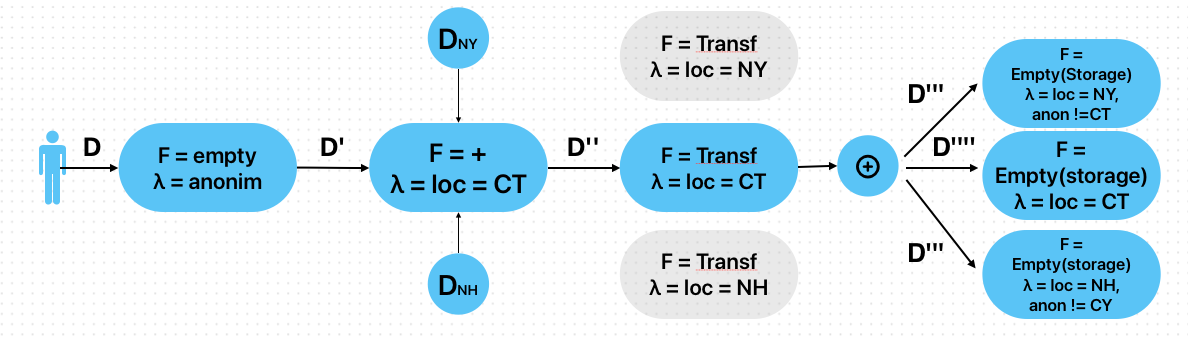
\includegraphics[width=0.98\columnwidth]{service_composition_example}
  \caption{Service composition example.}\label{fig:service_composition_example}

\end{figure}




\section{Pipeline Template}\label{sec:template}
Our approach integrates data protection and data management into the service pipeline using annotations. To this aim, we extend the service pipeline in \cref{def:pipeline} with: \emph{i)} data protection annotations that express transformations on data, ensuring compliance with data protection requirements, \emph{ii)} functional annotations that express data manipulations carried out during service execution.
These annotations enable the implementation of an advanced data lineage, tracking the entire data lifecycle by monitoring changes that result from functional service execution and data protection requirements.

In the following, we first introduce the annotated service pipeline, called pipeline template (Section \ref{sec:templatedefinition}). We then present both functional annotations (Section \ref{sec:funcannotation}) and data protection annotations (Section \ref{sec:nonfuncannotation}), providing an example of a pipeline template in the context of the reference scenario in Section \ref{sec:service_definition}.

\subsection{Pipeline Template Definition}\label{sec:templatedefinition}
Given the service pipeline in Definition~\ref{def:pipeline}, we use annotations to express data protection requirements and functional requirements on the services to be integrated in the pipeline. Each service vertex in the service pipeline is labeled with two mapping functions forming a pipeline template:
\begin{enumerate*}[label=\textit{\roman*})]
  \item an annotation function \myLambda:$\V_S\rightarrow$\P{} that associates a set of data protection requirements to be enforced on data, in the form of policies $p$$\in$\P{}, with each vertex \vi{i}$\in$$\V_S$;
  \item an annotation function \myGamma:$\V_S\rightarrow$\F{} that associates a functional service description $F_i\in\F{}$ with each vertex \vi{i}$\in$$\V_S$.
\end{enumerate*}

The template is formally defined as follows.

\vspace{0.5em}

\begin{definition}[Pipeline Template] \label{def:template}
  Given a service pipeline G(\V,\E), a Pipeline Template \tChartFunction is a direct acyclic graph extended with two annotation functions:
  \begin{enumerate}%[label=\textit{\roman*}]
    \item \emph{Data Protection Annotation} \myLambda that assigns a label \myLambda(\vi{i}) to each vertex $\vi{i}\in\V_S$. Label \myLambda(\vi{i}) corresponds to a set \P{i} of policies $p_j$ to be satisfied by service $s_i$ represented by \vi{i};
    \item \emph{Functional Annotation} \myGamma that assigns a label \myGamma(\vi{i}) to each vertex $\vi{i}\in\V_S$. Label \myGamma(\vi{i}) corresponds to the functional description $F_i$ of service $s_i$ represented by \vi{i}.
  \end{enumerate}
\end{definition}

\vspace{0.5em}

We note that, at this stage, the template is not yet linked to any service.
We also note that policies $p_j$$\in$\P{i} in \myLambda(\vi{i}) are combined using logical OR, meaning that the access decision is positive if at least one policy $p_j$ evaluates to \emph{true}.
% The pipeline template of the service pipeline of \cref{fig:reference_scenario} is depicted in \cref{fig:service_composition_template}.

      \subsection{Data Protection Annotation}\label{sec:nonfuncannotation}
      Data Protection Annotation \myLambda\ expresses data protection requirements in the form of access control policies. We consider an attribute-based access control model that offers flexible fine-grained authorization and adapts its standard key components to address the unique characteristics of a big data environment. Access requirements are expressed in the form of policy conditions that are defined as follows.

      \vspace{0.5em}

      \begin{definition}[Policy Condition]\label{def:policy_cond}
        A \emph{Policy Condition pc} is a Boolean expression of the form $($\emph{attr\_name} op \emph{attr\_value}$)$, with op$\in$\{$<$,$>$,$=$,$\neq$,$\leq$,$\geq$\}, \emph{attr\_name} an attribute label, and \emph{attr\_value} the corresponding attribute value.
      \end{definition}

      \vspace{0.5em}

      Built on policy conditions, an access control policy is then defined as follows.
      \vspace{0.5em}
      \begin{definition}[Policy]\label{def:policy_rule}
        A {\it policy p}$\in$\P{} is 5-uple $<$\textit{subj}, \textit{obj}, \textit{act}, \textit{env}, \textit{\TP}$>$ that specifies who (\emph{subject}) can access what (\emph{object}) with action (\emph{action}), in a specific context (\emph{environment}) and under specific obligations (\emph{data transformation}).
      \end{definition}

      \vspace{0.5em}

      More in detail, \textit{subject subj} specifies a service $s_i$ issuing an access request to perform an action on an object. It is a set \{$pc_i$\} of \emph{Policy Conditions} as defined in Definition \ref{def:policy_cond}. For instance, (classifier$=$``SVM'') specifies a service providing a SVM classifier. We note that \textit{subj} can also specify conditions on the service owner (\textit{e.g.}, owner\_location$=$``EU'') and the service user (\textit{e.g.}, service\_user\_role$=$``DOC Director'').

      \textit{Object obj} defines the data governed by the access policy. It is a set \{$pc_i$\} of \emph{Policy Conditions} on the object's attributes.
      For instance, \{(type$=$``dataset''), (region$=$``CT'')\} refers to an object of type dataset and whose region is Connecticut.

      \textit{Action act} specifies the operations that can be performed within a big data environment, from traditional atomic operations on databases (e.g., CRUD operations) to coarser operations, such as an Apache Spark Direct Acyclic Graph (DAG), Hadoop MapReduce, an analytics function call, and an analytics pipeline.

      \textit{Environment env} defines a set of conditions on contextual attributes, such as time of the day, location, IP address, risk level, weather condition, holiday/workday, and emergency. It is a set \{$pc_i$\} of \emph{Policy Conditions} as defined in Definition \ref{def:policy_cond}. For instance, (time$=$``night") refers to a policy that is applicable only at night.

      \textit{Data Transformation \TP} defines a set of security and privacy-aware transformations on \textit{obj} that must be enforced before any access to data is given. Transformations focus on data protection, as well as on compliance to regulations and standards, in addition to simple format conversions. For instance, let us define three transformations that can be applied to the dataset in \cref{tab:dataset}, each performing different levels of anonymization:
      \begin{enumerate*}[label=\roman*)]
        \item level \emph{l0} (\tp{0}): no anonymization;
        \item level \emph{l1} (\tp{1}): partial anonymization with only first and last name being anonymized;
        \item level \emph{l2} (\tp{2}): full anonymization with first name, last name, identifier and age being anonymized.
      \end{enumerate*}

Access control policies $p_j$$\in$\P{i} annotating a vertex \vi{i} in a pipeline template $G^{\myLambda,\myGamma}$ specify the data protection requirements that a candidate service must fulfill to be selected in the pipeline instance. Section~\ref{sec:instance} describes the selection process and the pipeline instance generation.

\subsection{Functional Annotations}\label{sec:funcannotation}
A proper data management approach must track functional data manipulations across the entire pipeline execution, defining the functional requirements of each service operating on data.
To this aim, each vertex \vi{i}$\in\V_S$ is annotated with a label \myGamma(\vi{i}), corresponding to the functional description $F_i$ of the service $s_i$ represented by \vi{i}.
$F_i$ describes the functional requirements, such as API, inputs, expected outputs.
It also specifies a set \TF{} of data transformation functions \tf{i}, which can be triggered during the execution of the corresponding service $s_i$.

Function $\tf{i}$$\in$$\TF{}$ can be:
\begin{enumerate*}[label=\textit{\roman*})]
  \item an empty function \tf{\epsilon} that applies no transformation or processing on the data;
  \item an additive function \tf{a} that expands the amount of data received, for example, by integrating data from other sources;
  \item a transformation function \tf{t} that transforms some records in the dataset without altering the domain;
  \item a transformation function \tf{d} (out of the scope of this work) that changes the domain of the data.
\end{enumerate*}

For simplicity but with no loss of generality, we assume that all candidate services meet functional annotation \F{} and that \TF{}=\tf{}. As a consequence, all candidate services apply the same transformation to the data during the pipeline execution.
\begin{table*}[!t]
  \def\arraystretch{1.5}
  \centering
  \caption{Anonymization policies (a) and data transformations (b)}\label{tab:anonymization}

  \resizebox{\textwidth}{!}{
    \begin{tabular}[t]{cc}
      \begin{tabular}[t]{c|c|l}
        \textbf{Vertex}      & \textbf{Policy} & \policy{subject}{object}{action}{environment}{transformation}                           \\ \hline
        \vi{1},\vi{2},\vi{3} & $\p{0}$         & \policy{ANY}{dataset}{READ}{ANY}{\tp{0}}                                                \\
        \vi{4},\vi{5}        & $\p{1}$         & \policy{\{\pone\}}{dataset}{READ}{ANY}{\tp{0}}                                              \\
        \vi{4},\vi{5}        & $\p{2}$         & \policy{\{\ptwo\}}{dataset}{READ}{ANY}{\tp{1}}                                              \\
        \vi{6}               & $\p{3}$         & \policy{\{$(service\_region=dataset\_origin)$\}}{dataset}{WRITE}{ANY}{\tp{0}} \\
        \vi{6}               & $\p{4}$         & \policy{\{$(service\_region=\{``NY",``NH"\})$\}}{dataset}{WRITE}{ANY}{\tp{1}}     \\
        \vi{7}               & $\p{5}$         & \policy{ANY}{dataset} {READ}{\langle$environment=``risky''$\rangle}{\tp{3}}                             \\
        \vi{7}               & $\p{6}$         & \policy{ANY}{dataset} {READ}{\langle$environment=``not\_risky''$\rangle}{\tp{4}}                        \\
      \end{tabular}
                        &

      \begin{tabular}[t]{c|c|l}
        \textbf{\tp{i}} & \textbf{Level} & \textbf{Data Transformation}                      \\\hline
        \tp{0}          & $l_0$          & $anon(\varnothing)$                               \\
        \tp{1}          & $l_1$          & $anon(fname, lname)$                              \\
        \tp{2}          & $l_2$          & $anon(fname, lname, id, age)$                     \\
        \tp{3}          & $r_0$          & $aggregation(cluster=\infty)                    $ \\
        \tp{4}          & $r_1$          & $aggregation(cluster=10)                       $  \\
        \multicolumn{3}{c}{\footnotesize (b)}
      \end{tabular} \\
      \footnotesize (a) &                                                                                          \\
    \end{tabular}
  }
\end{table*}

\begin{example}[\bf \pipelineTemplate]\label{ex:template}
Let us consider the reference scenario introduced in \cref{sec:systemmodel}.
\cref{fig:service_composition_template} presents an example of pipeline template consisting of five stages, each one annotated with a policy in \cref{tab:anonymization}.
{\color{OurColor}A visual aid to this example is presented in \cref{fig:pipeline_template_example}}.

% 1° NODO %
The first stage consists of three parallel vertices \vi{1}, \vi{2}, \vi{3} for data collection.
Data protection annotations \myLambda(\vi{1}), \myLambda(\vi{2}), \myLambda(\vi{3}) refer to policy \p{0} with an empty transformation \tp{0}.
Functional requirements \F{1}, \F{2}, \F{3}  prescribe a URI as input and the corresponding dataset as output.

The second stage consists of vertex \vi{4}, merging the three datasets obtained at the first stage. Data protection annotation \myLambda(\vi{4}) refers to policies \p{1} and \p{2}, which apply different data transformations depending on the relation between the dataset and the service owner.
% 2° NODO %
If the service owner is also the dataset owner (i.e., \pone), the dataset is not anonymized (\tp{0}). If the service owner is a partner of the dataset owner (i.e., \ptwo), the dataset is anonymized at \emph{level1} (\tp{1}). If the service owner has no partner relationship with the dataset owner, no policy applies.
Functional requirement \F{4} prescribes $n$ datasets as input and the merged dataset as output.

% 3° NODO %
The third stage consists of vertex \vi{5}  for data analysis.
Data protection annotation \myLambda(\vi{5}) refers to policies \p{1} and \p{2}, as for the second stage.
Functional requirement \F{5} prescribes a dataset as input and the results of the data analysis as output.

% 5° NODO %
The fourth stage consists of vertex \vi{6}, managing data storage. Data protection annotation \myLambda(\vi{6}) refers to policies \p{3} and \p{4}, which apply different data transformations depending on the relation between the dataset and the service region.
If the service region is the dataset origin (condition $(service\_region$$=$$dataset\_origin)$ in \p{3}), the dataset is anonymized at level $l_0$ (\tp{0}).
If the service region is in a partner region (condition ($service\_region$=\{``$NY$",``$NH$"\}) in \p{4}), the dataset is anonymized at level $l_1$ (\tp{1}).
Functional requirement \F{7} prescribes a dataset as input and the URI of the stored data as output.

% 6° NODO %
The last stage consists of vertex \vi{7}, responsible for data visualization.
Data protection annotation \myLambda(\vi{7}) refers to policies \p{5} and \p{6}, which anonymize data according to the environment where the service is executed.
A \emph{risky} environment is defined as a region outside the owner or partner facility.
If the environment is risky (\p{5}), the data are anonymized at level $r_0$ (\tp{3}).
If the environment is not risky (\p{6}), the data are anonymized at level $r_1$ (\tp{4}).
Functional requirement \F{8} prescribes a dataset as input and data visualization interface (possibly in the form of JSON file) as output.
\end{example}

\begin{figure}
  \centering
  % \resizebox{\columnwidth}{!}{%
  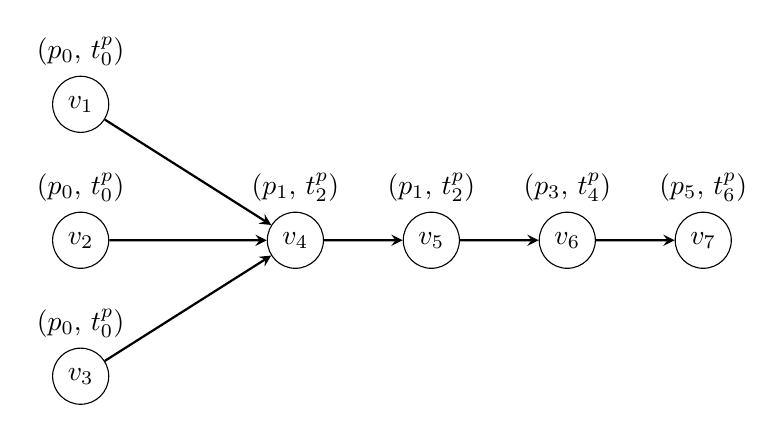
\begin{tikzpicture}[
    box/.style={draw, circle},
    arrow/.style={->, >=stealth, thick},
    scale=0.9
]
% Nodes for the stages
\node[box] (v1) {$\vi{1}$};
\node[box, below=of v1] (v2) {$\vi{2}$};
\node[box, below=of v2] (v3) {$\vi{3}$};
\node[box, right=of v2, xshift=1cm] (v4) {$\vi{4}$};
\node[box, right=of v4] (v5) {$\vi{5}$};
\node[box, right=of v5] (v6) {$\vi{6}$};
\node[box, right=of v6] (v7) {$\vi{7}$};

\node[above] at (v1.north)  {(\p{0}, \tp{0})};
\node[above] at (v2.north)  {(\p{0}, \tp{0})};
\node[above] at (v3.north)  {(\p{0}, \tp{0})};
\node[above] at (v4.north)  {(\p{1}, \tp{2})};
\node[above] at (v5.north)  {(\p{1}, \tp{2})};
\node[above] at (v6.north)  {(\p{3}, \tp{4})};
\node[above] at (v7.north)  {(\p{5}, \tp{6})};
% Arrows connecting the stages
\draw[arrow] (v1) -- (v4);
\draw[arrow] (v2) -- (v4);
\draw[arrow] (v3) -- (v4);
\draw[arrow] (v4) -- (v5);
\draw[arrow] (v5) -- (v6);
\draw[arrow] (v6) -- (v7);

\end{tikzpicture}
  % }
  \caption{\label{fig:pipeline_template_example}Example of pipeline template}
\end{figure}
\section{Pipeline Instance}\label{sec:instance}
%Given a set of candidate services, a
A \pipelineInstance $\iChartFunction$ instantiates a \pipelineTemplate \tChartFunction by composing services in the instance according to data protection and functional annotations in the template.  It is formally defined as follows.

\begin{definition}[Pipeline Instance]\label{def:instance}
  Let \tChartFunction be a pipeline template, a pipeline Instance $\iChartFunction$ is an isomorphic directed acyclic graph where:
  \begin{enumerate*}[label=\textit{\roman*})]
    \item $v'_r$$=$$v_r$;
    \item for each vertex $\vi{}\in\V_{\timesOperator}\cup\V_{\plusOperator}$, there exists a corresponding vertex $\vii{}\in\Vp_{\timesOperator}\cup\Vp_{\plusOperator}$;
    \item for each $\vi{i}$$\in$$\V_S$ annotated with policy \P{i}, there exists a corresponding vertex \vii{i}$\in$$\Vp_S$ instantiated with a service \sii{i}, such that:
  \end{enumerate*}
  \begin{enumerate}[label=\arabic*)]
    \item $s'_i$ satisfies data protection annotation \myLambda(\vi{i}) in \tChartFunction;
    \item $s'_i$ satisfies functional annotation \myGamma(\vi{i}) in \tChartFunction.
  \end{enumerate}
\end{definition}

Condition 1 requires that each selected service \sii{i} satisfies the policy requirements \P{i} of the corresponding vertex \vi{i} in the \pipelineTemplate, whereas Condition 2 is needed to preserve the process functionality, as it simply states that each service \sii{i} must satisfy the functional requirements \F{i} of the corresponding vertex \vi{i} in the \pipelineTemplate.

We then define a \emph{pipeline instantiation} function that takes as input a \pipelineTemplate \tChartFunction and a set $S^c$ of candidate services, with a specific set of services $S^c_{i}$ for each vertex \vi{i}$\in$$\V_S$, and returns as output a \pipelineInstance \iChartFunction. Recall from Section~\ref{sec:funcannotation} that all candidate services meet the functional annotation in the template, meaning that Condition 2 in Definition~\ref{def:instance} is satisfied for all candidate services.

    The \pipelineInstance  is generated by traversing the \pipelineTemplate with a breadth-first search algorithm, starting from the root vertex \vi{r}.
    Then, for each vertex $v\in\Vplus\bigcup\Vtimes$ in the pipeline template, the corresponding vertex $v'\in\Vpplus\bigcup\Vptimes$ is generated.
    Finally, for each vertex \vi{i}$\in$$\V_S$, a two-step approach is applied as follows.

  \begin{enumerate}

    \item \textit{Filtering Algorithm} -- The filtering algorithm checks if the profile \profile$_j$ of each candidate service $\si{j}$$\in$$S^c_{i}$ satisfies the policies $p_k$$\in$\P{i} corresponding to \myLambda(\vi{i}). If \profile$_j$ satisfies at least one policy,  service $\si{j}$ is compatible, otherwise it is discarded. The filtering algorithm finally returns a subset $S'_{i}$$\subseteq$$S^c_{i}$ of compatible services for each vertex \vi{i}$\in$$\V_S$.
    \item \textit{Selection Algorithm} -- The selection algorithm selects one service $s'_i$ for each set $S'_{i}$ of compatible services and instantiates the corresponding vertex $\vii{i}$$\in$$\Vp$ with it. There are many ways of choosing $s'_i$, we present our approach based on the minimization of quality loss in Section \ref{sec:metrics}.
  \end{enumerate}

  When all vertices $\vi{i}$$\in$$V$ have been visited, the \pipelineInstance G' is finalized, with a service instance $s'_i$ for each \vii{i}$\in$\Vp. Vertex \vii{i} is still annotated with policies $p_k$$\in$\P{i} according to \myLambda, because policies in \P{i} are evaluated and enforced only when the pipeline instance is triggered, before any service is executed. In case policy evaluation returns \emph{true}, data transformation \TP$\in$\P{i} is applied, otherwise a default transformation that removes all data is applied.

\begin{figure}[ht!]
  \centering
  \newcommand{\function}[1]{$\instanceChartAnnotation{}_{#1}$}
  \begin{tikzpicture}[scale=0.7]
    % vertexes
    \node[draw, circle, fill,text=white,minimum size=1 ] (sr) at (0,0) {};

    % \node[draw, circle] (node2) at (1,0) {$\s{1}$};
    \node[draw, circle, plus,minimum size=1.5em] (plus) at (1.5,0) {};

    \node[draw, circle] (s2) at (3.5,-2) {$\sii{1}$};
    \node[draw, circle] (s3) at (3.5,0) {$\sii{2}$};
    \node[draw, circle] (s1) at (3.5,2) {$\sii{3}$};

    \node[draw, circle] (s4) at (5,0) {$\sii{4}$};
    \node[draw, circle] (s5) at (6.5,0) {$\sii{5}$};

    \node[draw, circle] (s6) at (8.0,0) {$\sii{6}$};
    \node[draw, circle] (s7) at (9.5,0) {$\sii{7}$};
    % Text on top
    % \node[above] at (sr.north)  {\function{}};
    \node[above] at (s1.north)  {\function{3}};

    \node[above] at (s2.north)  {\function{1}};
    \node[above] at (s3.north)  {\function{2}};
    \node[above] at (s4.north)  {\function{4}};
    \node[above] at (s5.north)  {\function{5}};
    % \node[above] at (s6.north)  {\function{}};
    \node[above] at (s6.north)  {\function{6}};
    \node[above] at (s7.north)  {\function{7}};
    % Connection

    % \draw[->] (node2) -- (node3);
    \draw[->] (sr) -- (plus);
    \draw[->] (plus) -- (s1);
    \draw[->] (plus) -- (s2);
    \draw[->] (plus) -- (s3);

    \draw[->] (s1) -- (s4);
    \draw[->] (s2) -- (s4);
    \draw[->] (s3) -- (s4);
    % \draw[->] (node6) -- (node65);
    % \draw[->] (node65) -- (node7);3
    \draw[->] (s4) -- (s5);
    \draw[->] (s5) -- (s6);
    % \draw[->] (cross) -- (s5);
    % \draw[->] (cross) -- (s6);
    % \draw[->] (s5) -- (s7);
    % \draw[->] (s6) -- (s7);
    \draw[->] (s6) -- (s7);

  \end{tikzpicture}
  \caption{Service composition instance}
  \label{fig:service_composition_instance}
\end{figure}


% \subsection{Pipeline Instance Definition}\label{sec:instancedefinition}
% The goal of our approach is to generate an instance of the \pipelineTemplate starting from the \pipelineTemplate in Section~\ref{sec:template}. In the following, we first define the pipeline instance and the corresponding pipeline instantiation process (Section \ref{sec:instancedefinition}). We then prove that the pipeline instantiation process is NP-hard (Section \ref{sec:funcannotation}).

% \subsection{Pipeline Instance Definition}\label{sec:instancedefinition}
% A \pipelineInstance $\iChartFunction$ is a ready-to-be-executed pipeline, which instantiates a \pipelineTemplate \tChartFunction \chia{ selecting the services} according to its data protection and functional annotations. We formally define \tChartFunction as follows.

%     \begin{definition}[Pipeline Instance]\label{def:instance}
%       Let \tChartFunction be a Pipeline Template, a Pipeline Instance $\iChartFunction$ is a directed acyclic graph where:
%       \begin{enumerate*}[label=\textit{\roman*})]
%         \item $s_r$$=$$s'_r$;
%         \item for each vertex $\vi{}\in\V_{\timesOperator}\cup\V_{\plusOperator}$ it exists a corresponding vertex $\vii{}\in\Vp_{\timesOperator}\cup\Vp_{\plusOperator}$;
%         \item for each $\vi{i}$$\in$$\V_S$ annotated with policy \P{i} it exists a corresponding \vii{i}$\in$$\Vp_S$ instantiated with a service instance \sii{i};
%       \end{enumerate*}
%       and such that the following conditions hold:
%       \begin{enumerate}[label=\arabic*)]
%         \item $s'_i$ satisfies data protection annotation \myLambda(\vi{i}) in \tChartFunction;
%         \item $s'_i$ satisfies functional annotation \myGamma(\vi{i}) in \tChartFunction.
%       \end{enumerate}
%     \end{definition}

% Condition 1 states that each service \sii{i} must satisfy the policy requirements \P{i} of the corresponding vertex \vi{i} in the \pipelineTemplate.
%     Condition 2 is needed to preserve the process functionality, as it simply states that each service \sii{i} must satisfy the functional requirements \F{i} of the corresponding vertex \vi{i} in the \pipelineTemplate.

%     We recall that Condition 2 is satisfied for all candidate services (see Section~\ref{sec:funcannotation}) and therefore concentrate on Condition 1 in the following.

% We then define a \emph{Pipeline Instantiation Process} as a function that takes as input a \pipelineTemplate \tChartFunction and a set $S^c$ of candidate services, one for each vertex \vi{i}$\in$\V,\marginpar{ \chia{ $\V_S$?}} and returns as output a \pipelineInstance \iChartFunction in Definition~\ref{def:instance}.
%     %In \iChartFunction, every invocations \vii{i}$\in$$V'_S$ contains a service instance, and every branching $v\in\Vplus\bigcup\Vtimes$ in the template is maintained as is.
%  \chia{ The objective of the Pipeline Instantiation Process is to return a Pipeline Instance that minimizes the quantity of information lost, and maximizes the level of data protection and data sharing, not for the selection of a single service, but in the overall. To this aim, the  \pipelineTemplate is traversed with a breadth-first search algorithm and for each vertex \vi{i}$\in$$\V_S$, a two-step selection approach is applied as follows.}

% %Ovviamente non è sufficiente scegliere il best service per ogni vertice, ma diventa un problema complesso dove si devono calcolare/valutare tutte le possibili combinazioni dei servizi disponibili, tra le quali scegliere la migliore.

%     The \pipelineInstance  is generated by traversing the \pipelineTemplate with a breadth-first search algorithm, starting from the root vertex \vi{r}.
%     Then, for each vertex $v\in\Vplus\bigcup\Vtimes$ in the pipeline template, the corresponding vertex $v'\in\Vpplus\bigcup\Vptimes$ is generated.
%     Finally, for each vertex \vi{i}$\in$$\V_S$, a two-step selection approach is applied as follows.

% \subsection{Pipeline Instance - VECCHIO PARAGRAFO}\label{sec:instance}
% %The goal of our approach is to generate \pipelineInstance starting from the \pipelineTemplate in Section~\ref{sec:template}.
% A \pipelineInstance $\iChartFunction$ instantiates a \pipelineTemplate \tChartFunction by selecting the component services according to its data protection and functional annotations. We formally define \tChartFunction as follows.

%     \begin{definition}[Pipeline Instance]\label{def:instance}
%       Let \tChartFunction be a pipeline template, a pipeline Instance $\iChartFunction$ is a directed acyclic graph where:
%       \begin{enumerate*}[label=\textit{\roman*})]
%         \item $s_r$$=$$s'_r$;
%         \item for each vertex $\vi{}\in\V_{\timesOperator}\cup\V_{\plusOperator}$ it exists a corresponding vertex $\vii{}\in\Vp_{\timesOperator}\cup\Vp_{\plusOperator}$;
%         \item for each $\vi{i}$$\in$$\V_S$ annotated with policy \P{i} it exists a corresponding \vii{i}$\in$$\Vp_S$ instantiated with a service instance \sii{i};
%       \end{enumerate*}
%       and such that the following conditions hold:
%       \begin{enumerate}[label=\arabic*)]
%         \item $s'_i$ satisfies data protection annotation \myLambda(\vi{i}) in \tChartFunction;
%         \item $s'_i$ satisfies functional annotation \myGamma(\vi{i}) in \tChartFunction.
%       \end{enumerate}
%     \end{definition}

% Condition 1 states that each service \sii{i} must satisfy the policy requirements \P{i} of the corresponding vertex \vi{i} in the \pipelineTemplate.
% Condition 2 is needed to preserve the process functionality, as it simply states that each service \sii{i} must satisfy the functional requirements \F{i} of the corresponding vertex \vi{i} in the \pipelineTemplate. We recall that Condition 1 is satisfied for all candidate services (see Section~\ref{sec:funcannotation}) and therefore concentrate on Condition 2 in the following.

%     We then define a \emph{pipeline instantiation} function that takes as input a \pipelineTemplate \tChartFunction and a set $S^c$ of candidate services, one for each vertex \vi{i}$\in$$\V_S$, and returns as output a \pipelineInstance \iChartFunction in Definition~\ref{def:instance}.
%        %In \iChartFunction, every invocations \vii{i}$\in$$V'_S$ contains a service instance, and every branching $v\in\Vplus\bigcup\Vtimes$ in the template is maintained as is.
%     %\chia{ The objective of the Pipeline Instantiation Process is to return a Pipeline Instance that minimizes the quantity of information lost, and maximizes the level of data protection and data sharing, not for the selection of a single service, but in the overall. To this aim, the  \pipelineTemplate is traversed with a breadth-first search algorithm and for each vertex \vi{i}$\in$$\V_S$, a two-step selection approach is applied as follows.}
%   %
%   % %Ovviamente non è sufficiente scegliere il best service per ogni vertice, ma diventa un problema complesso dove si devono calcolare/valutare tutte le possibili combinazioni dei servizi disponibili, tra le quali scegliere la migliore.
%      %
%     The \pipelineInstance  is generated by traversing the \pipelineTemplate with a breadth-first search algorithm, starting from the root vertex \vi{r}.
%     Then, for each vertex $v\in\Vplus\bigcup\Vtimes$ in the pipeline template, the corresponding vertex $v'\in\Vpplus\bigcup\Vptimes$ is generated.
%     Finally, for each vertex \vi{i}$\in$$\V_S$, a two-step selection approach is applied as follows.

%   \begin{itemize}

%     \item \textit{Filtering Algorithm} -- As already discussed in Section~\ref{sec:templatedefinition}, the filtering algorithm retrieves a set of candidate services $S^c$ and matches them one-by-one against data protection requirements \myLambda(\vi{i}). In particular, the profile of each candidate service \si{j} is matched against policies $p_k$$\in$\P{i} corresponding to \myLambda(\vi{i}). Filtering algorithm returns as output the set of compatible services that match the policy.

%     Formally, let us consider a set $S^c$ of candidate services \si{j}, each one having a profile as a set of attributes in the form (\emph{name}, \emph{value}). The filtering algorithm is executed for each \si{j}; it is successful if \si{j}'s profile satisfies at least one policy $p_k$$\in$\P{i}; otherwise, \si{j} is discarded and not considered for selection. The filtering algorithm finally returns a subset $S'\subseteq S^c$ of compatible services, among which the service instance is selected.

%     \item \textit{Selection Algorithm} -- Upon retrieving a set $S'$ of compatible services \si{j}, a service $s'_i$$\in$$S'$ is then selected and integrated in $\vii{i}\in \Vp$. There are many ways of choosing $s'_i$, we present our approach based on quality loss in Section \ref{sec:metrics}.
%     %\item \textit{Selection Algorithm} -- Upon retrieving a set $S'$ of compatible services \si{j}, it produces a ranking of these services according to some metrics that evaluates the quality loss introduced by each service when integrated in the pipeline instance. More details about the metrics are provided in Section \ref{sec:metrics}. The best service $s'_i$ is then selected and integrated in $\vii{i}\in \Vp$. There are many ways of choosing relevant metrics, we present those used in this article in Section \ref{sec:metrics}.
%   \end{itemize}

%   When all vertices $\vi{i}\in V$ have been visited, a \pipelineInstance G' is generated, where each \vii{i}$\in$\Vp contains a service instance $s'_i$. We note that each vertex \vii{i} is annotated with policies $p_k$$\in$\P{i} according to \myLambda. When pipeline instance is triggered, before any services can be executed, policies in \P{i} are evaluated and enforced. In case policy evaluation returns \emph{true}, data transformation \TP$\in$\P{i} is applied, otherwise a default transformation that removes all data is applied.

% \begin{figure}[ht!]
%   \centering
%   \newcommand{\function}{$\instanceChartAnnotation{}$}
%   \begin{tikzpicture}[scale=0.7]
%     % vertexes
%     \node[draw, circle] (sr) at (0,0) {$\vi{r}$};
%     % \node[draw, circle] (node2) at (1,0) {$\s{1}$};
%     \node[draw, circle, plus,minimum size=1.5em] (plus) at (1.5,0) {};
%     \node[draw, circle] (s1) at (3,1.7) {$\sii{1}$};
%     \node[draw, circle] (s2) at (3,-1.7) {$\sii{2}$};
%     \node[draw, circle] (s3) at (3,0) {$\sii{3}$};


%     \node[draw, circle] (s4) at (4.5,0) {$\sii{4}$};
%     \node[draw, circle, cross,minimum size=1.5em] (cross) at (6,0) {};
%     \node[draw, circle] (s5) at (7.5,1.2) {$\sii{5}$};
%     \node[draw, circle] (s6) at (7.5,-1.2) {$\sii{6}$};

%     \node[draw, circle] (s7) at (9,0) {$\sii{7}$};
%     \node[draw, circle] (s8) at (10.5,0) {$\sii{8}$};
%     % Text on top
%     \node[above] at (sr.north)  {\function{}};
%     \node[above] at (s1.north)  {\function{}};

%     \node[above] at (s2.north)  {\function{}};
%     \node[above] at (s3.north)  {\function{}};
%     \node[above] at (s4.north)  {\function{}};
%     \node[above] at (s5.north)  {\function{}};
%     \node[above] at (s6.north)  {\function{}};
%     \node[above] at (s7.north)  {\function{}};
%     \node[above] at (s8.north)  {\function{}};
%     % Connection

%     % \draw[->] (node2) -- (node3);
%     \draw[->] (sr) -- (plus);
%     \draw[->] (plus) -- (s1);
%     \draw[->] (plus) -- (s2);
%     \draw[->] (plus) -- (s3);

%     \draw[->] (s1) -- (s4);
%     \draw[->] (s2) -- (s4);
%     \draw[->] (s3) -- (s4);
%     % \draw[->] (node6) -- (node65);
%     % \draw[->] (node65) -- (node7);3
%     \draw[->] (s4) -- (cross);
%     \draw[->] (cross) -- (s5);
%     \draw[->] (cross) -- (s6);
%     \draw[->] (s5) -- (s7);
%     \draw[->] (s6) -- (s7);
%     \draw[->] (s7) -- (s8);

%   \end{tikzpicture}
%   \caption{Service composition instance}
%   \label{fig:service_composition_instance}
% \end{figure}


% % \subsection{Pipeline Instance Definition}\label{sec:instancedefinition}
%   % The goal of our approach is to generate an instance of the \pipelineTemplate starting from the \pipelineTemplate in Section~\ref{sec:template}. In the following, we first define the pipeline instance and the corresponding pipeline instantiation process (Section \ref{sec:instancedefinition}). We then prove that the pipeline instantiation process is NP-hard (Section \ref{sec:funcannotation}).

%   % \subsection{Pipeline Instance Definition}\label{sec:instancedefinition}
%   % A \pipelineInstance $\iChartFunction$ is a ready-to-be-executed pipeline, which instantiates a \pipelineTemplate \tChartFunction \chia{ selecting the services} according to its data protection and functional annotations. We formally define \tChartFunction as follows.

%   %     \begin{definition}[Pipeline Instance]\label{def:instance}
%   %       Let \tChartFunction be a Pipeline Template, a Pipeline Instance $\iChartFunction$ is a directed acyclic graph where:
%   %       \begin{enumerate*}[label=\textit{\roman*})]
%   %         \item $s_r$$=$$s'_r$;
%   %         \item for each vertex $\vi{}\in\V_{\timesOperator}\cup\V_{\plusOperator}$ it exists a corresponding vertex $\vii{}\in\Vp_{\timesOperator}\cup\Vp_{\plusOperator}$;
%   %         \item for each $\vi{i}$$\in$$\V_S$ annotated with policy \P{i} it exists a corresponding \vii{i}$\in$$\Vp_S$ instantiated with a service instance \sii{i};
%   %       \end{enumerate*}
%   %       and such that the following conditions hold:
%   %       \begin{enumerate}[label=\arabic*)]
%   %         \item $s'_i$ satisfies data protection annotation \myLambda(\vi{i}) in \tChartFunction;
%   %         \item $s'_i$ satisfies functional annotation \myGamma(\vi{i}) in \tChartFunction.
%   %       \end{enumerate}
%   %     \end{definition}

%   % Condition 1 states that each service \sii{i} must satisfy the policy requirements \P{i} of the corresponding vertex \vi{i} in the \pipelineTemplate.
%   %     Condition 2 is needed to preserve the process functionality, as it simply states that each service \sii{i} must satisfy the functional requirements \F{i} of the corresponding vertex \vi{i} in the \pipelineTemplate.

%   %     We recall that Condition 2 is satisfied for all candidate services (see Section~\ref{sec:funcannotation}) and therefore concentrate on Condition 1 in the following.

%   % We then define a \emph{Pipeline Instantiation Process} as a function that takes as input a \pipelineTemplate \tChartFunction and a set $S^c$ of candidate services, one for each vertex \vi{i}$\in$\V,\marginpar{ \chia{ $\V_S$?}} and returns as output a \pipelineInstance \iChartFunction in Definition~\ref{def:instance}.
%   %     %In \iChartFunction, every invocations \vii{i}$\in$$V'_S$ contains a service instance, and every branching $v\in\Vplus\bigcup\Vtimes$ in the template is maintained as is.
%   %  \chia{ The objective of the Pipeline Instantiation Process is to return a Pipeline Instance that minimizes the quantity of information lost, and maximizes the level of data protection and data sharing, not for the selection of a single service, but in the overall. To this aim, the  \pipelineTemplate is traversed with a breadth-first search algorithm and for each vertex \vi{i}$\in$$\V_S$, a two-step selection approach is applied as follows.}

%   % %Ovviamente non è sufficiente scegliere il best service per ogni vertice, ma diventa un problema complesso dove si devono calcolare/valutare tutte le possibili combinazioni dei servizi disponibili, tra le quali scegliere la migliore.

%   %     The \pipelineInstance  is generated by traversing the \pipelineTemplate with a breadth-first search algorithm, starting from the root vertex \vi{r}.
%   %     Then, for each vertex $v\in\Vplus\bigcup\Vtimes$ in the pipeline template, the corresponding vertex $v'\in\Vpplus\bigcup\Vptimes$ is generated.
%   %     Finally, for each vertex \vi{i}$\in$$\V_S$, a two-step selection approach is applied as follows.




\begin{example}\label{ex:instance}

  As an example, let us consider the pipeline template \tChartFunction in \cref{sec:example}.
  It includes three key stages in our reference scenario: data anonymization (\vi{1}), data enrichment (\vi{2}), and data aggregation (\vi{3}), each stage with its policy $p$.



  The filtering algorithm then returns the set $S'=\{s_1,s_2\}$.
  The comparison algorithm is finally applied to $S'$ and returns a ranking of the services according to quality metrics, where $s_1$ is ranked first. $s_1$ is then selected and integrated in $\vii{1}\in \Vp$.

  The comparison algorithm is finally applied to $S'$ and returns a ranking of the services according to quality metrics, where $s_1$ is ranked first. $s_1$ is then selected and integrated in $\vii{1}\in \Vp$.

  The same logic is applied to the \vi{2} and \vi{3}.

\end{example}
\section{Maximizing the Pipeline Instance Quality}\label{sec:heuristics}
%
% %Ovviamente non è sufficiente scegliere il best service per ogni vertice, ma diventa un problema complesso dove si devono calcolare/valutare tutte le possibili combinazioni dei servizi disponibili, tra le quali scegliere la migliore.
Our goal is to generate a pipeline instance with maximum quality \q, addressing data protection requirements throughout the pipeline execution. To this aim, we first discuss the quality metrics used to measure and monitor data quality \q, which guide the generation of the pipeline instance with maximum \q. Then, we prove that the problem of generating a pipeline instance with maximum \q\ is NP-hard (\cref{sec:nphard}). Finally, we introduce a parametric heuristic (\cref{subsec:heuristics}) designed to tackle the computational complexity associated with enumerating all possible combinations within a given set. The main objective of the heuristic is to approximate the optimal path for service interactions and transformations, especially within the realm of complex pipelines consisting of numerous vertices and candidate services. Our focus extends beyond identifying optimal combinations to include an understanding of the quality changes introduced during the transformation processes.

%Inspired by existing literature, these metrics, categorized as quantitative and statistical, play a pivotal role in quantifying the impact of policy-driven transformations on the original dataset.

\subsection{Quality Metrics}\label{subsec:metrics}
%Ensuring data quality is mandatory to implement data pipelines that provide accurate results and decision-making along the whole pipeline execution. To this aim, we define two metrics evaluating the quality loss introduced by our policy-driven transformation in Section~\cite{ADD} on the input dataset \origdataset at each step of the data pipeline. Our metrics can be classified as \emph{quantitative} and \emph{qualitative}~\cite{ADD}, and compare the input dataset \origdataset\ and dataset \transdataset\ generated by enforcing data protection requirements on \origdataset.
Ensuring data quality is mandatory to implement data pipelines that provide accurate results and decision-making along the whole pipeline execution. Quality metrics measure the data quality preserved at each step of the data pipeline, and can be classified as \emph{quantitative} or \emph{qualitative}. %~\cite{ADD}\hl{CITE}.
Quantitative metrics monitor the amount of data lost during data transformations to model the quality difference between datasets \origdataset\ and \transdataset.
Qualitative metrics evaluate changes in the properties of datasets \origdataset\ and \transdataset. For instance, qualitative metrics can measure the changes in the statistical distribution of the two datasets.

In this paper, we use two metrics, one quantitative and one qualitative, to compare the input dataset \origdataset\ and dataset \transdataset\ generated by enforcing data protection requirements (i.e., our policy-driven transformation in \cref{sec:instance}) on \origdataset\ at each step of the pipeline. We note that a complete taxonomy of possible metrics is outside the scope of this paper and will be the target of our future work.

\subsubsection{Quantitative metric}
%We propose a metric that measures the similarity between two datasets, for this purpose, we use the Jaccard coefficient.
We propose a quantitative metric $M_J$ based on the Jaccard coefficient that assesses the similarity between two datasets. The Jaccard coefficient is defined as follows \cite{RAHMAN20102707}: \[J(X,Y) = \frac{|X \cap Y|}{|X \cup Y|}\]
where X and Y are two datasets of the same size.

The coefficient is calculated by dividing the cardinality of the intersection of two datasets by the cardinality of their union. It ranges from 0 to 1, with 0 indicating no similarity (minimum quality) and 1 indicating complete similarity (maximum quality) between the datasets. It has several advantages. Unlike other similarity measures, such as Euclidean distance, it is not affected by the magnitude of the values in the dataset. It is suitable for datasets with categorical variables or nominal data, where the values do not have a meaningful numerical interpretation.

Metric $M_J$ extends the Jaccard coefficient with weights that model the importance of each element in the dataset as follows:\[M_J(X,Y) = \frac{\sum_{i=1}^{n}w_i(x_i \cap y_i)}{\sum_{i=1}^{n}w_i(x_i \cup y_i)}\]
where $x_i$$\in$X ($y_i$$\in$Y, resp.) is the $i$-th feature of dataset X (Y, resp.), and $w_i$ the weight modeling the importance of the $i$-th feature.

It is computed by dividing the cardinality of the intersection of two datasets by the cardinality of their union, weighted by the importance of each feature in the datasets. It provides a more accurate measure of similarity. %Weights prioritize certain elements (e.g., a specific feature) in the datasets.
%The Weighted Jaccard coefficent can then account for element importance and provide a more accurate measure of similarity.

\subsubsection{Qualitative Metric}
%We propose a metric that enables the measurement of the distance of two distributions.
We propose a qualitative metric $M_{JSD}$ based on the Jensen-Shannon Divergence (JSD) that assesses the similarity (distance) between the probability distributions of two datasets.

JSD is a symmetrized version of the KL divergence~\cite{Fuglede} and is applicable to a pair of statistical distributions only. It is defined as follows:
\[JSD(X, Y) = \frac{1}{2} \left( KL(X || M)
  + KL(Y || M) \right)\]
%
where X and Y are two distributions of the same size, and M$=$0.5*(X+Y) is the average distribution.
JSD incorporates both the KL divergence from X to M and from Y to M.

To make JSD applicable to datasets, where each feature in the dataset has its own statistical distribution, metric $M_{JSD}$ applies JSD to each column of the dataset. The obtained results are then aggregated using a weighted average, thus enabling the prioritization of important features that can be lost during the policy-driven transformation in \cref{sec:heuristics}, as follows: \[M_{JSD} = 1 - \sum_{i=1}^n w_i \cdot \text{JSD}(x_i,y_i)\]
%where \(w_i = \frac{n_i}{N}\) represents the weight for the \(i\)-th column, with \(n_i\) being the number of distinct elements in the $i$-th feature and \(N\) the total number of elements in the dataset.
where $\sum_{i=1}^n w_i$$=$1 and each \(\text{JSD}(x_i,y_i)\) accounts for the Jensen-Shannon Divergence computed for the \(i\)-th feature in datasets X and Y. It ranges from 0 to 1, with 0 indicating no similarity (minimum quality) and 1 indicating complete similarity (maximum quality) between the datasets.
%Must be noted that the one minus has been added to the formula to transfrom the metric into a similarity metric, where 1 indicates complete similarity and 0 indicates no similarity.

$M_{JSD}$ provides a weighted measure of similarity, which is symmetric and accounts for the contribution from both datasets and specific features. It can compare the similarity of the two datasets, providing a symmetric and normalized measure that considers the overall data distributions.


\subsubsection{Pipeline Quality}
%We note that our metrics can be applied either to the entire dataset or to specific features only. The features can be assigned with equal or varying importance, providing a weighted version of the metrics, thus enabling the prioritization of important features that might be possibly lost during the policy-driven transformation in Section~\cite{ADD}.

Metrics $M_J$ and $M_{JSD}$ contribute to the calculation of the pipeline quality \q\ as follows. %Information loss is calculated as the average \emph{AVG} of data at each vertex \vi{i}$\in$$\V_S$ of the service pipeline $G(V,E)$ as follows.

\vspace{0.5em}

\begin{definition}[\emph{\quality}]\label{def:quality}
  Given a metric $M$$\in$$\{M_J,M_{JSD}$\} modeling the data quality, pipeline quality \q$=$$M_{ij}$, with $M_{ij}$ the value of the quality metric retrieved at each vertex \vii{i}$\in$$\V'_S$ of the pipeline instance $G'$ according to service \sii{j}.
\end{definition}

\vspace{0.5em}

We note that $M_{ij}$ models the average data quality preserved within the pipeline instance $G'$.
We also note that $\q_{ij}$$=$$M_{ij}$ models the \quality at vertex \vii{i}$\in$$\V'_S$ of $G'$ for \sii{j}.
%We also note that information loss \textit{dloss} is used to generate the Max-Quality pipeline instance in the remaining of this section.

\subsection{NP-Hardness of the Max-Quality Pipeline Instantiation Problem}\label{sec:nphard}
%\hl{se lo definiamo in maniera formale come il problema di trovare un'istanza valida in accordo alla definizione di istanza tale che non ne esiste una con un loss piu' piccolo?}
The problem of computing a pipeline instance (\cref{def:instance}) with maximum quality \q\ can be formally defined as follows.

\vspace{0.5em}

\begin{definition}[Max-Quality Problem]\label{def:MaXQualityInstance}
  Given a pipeline template $G^{\myLambda,\myGamma}$ and a set $S^c$ of candidate services, find a max-quality pipeline instance $G'$ such that:
  \begin{itemize}
    \item $G'$ satisfies conditions in \cref{def:instance},
    \item $\nexists$ a pipeline instance $G''$ that satisfies conditions in \cref{def:instance} and such that quality \q($G''$)$>$\q($G'$), where \q($\cdot$) is the pipeline quality in Definition~\ref{def:quality}.
    %computed after applying the transformation of the policy matching the service selected to instantiate vertex  \vi{i}$\in$$\V_S$, .
  \end{itemize}
\end{definition}

\vspace{0.5em}

The Max Quality \problem is a combinatorial selection problem and is NP-hard, as stated by Theorem \cref{theorem:NP}. However, while the overall problem is NP-hard, there is a component of the problem that is solvable in polynomial time: matching the profile of each service with the corresponding vertex policy. This can be done by iterating over each vertex and each service, checking if the service matches the vertex policy. This process takes polynomial time complexity $O(|N|*|S|)$.

\vspace{0.5em}

\begin{theorem}\label{theorem:NP}
  The Max-Quality \problem is NP-Hard.
\end{theorem}
\emph{Proof: }
The proof is a reduction from the multiple-choice knapsack problem (MCKP), a classified NP-hard combinatorial optimization problem, which is a generalization of the simple knapsack problem (KP) \cite{}\hl{CITA}. In the MCKP problem, there are $t$ mutually disjoint classes $N_1,N_2,\ldots,N_t$ of items to pack in some knapsack of capacity $C$, class $N_i$ having size $n_i$. Each item $j$$\in$$N_i$ has a profit $p_{ij}$ and a weight $w_{ij}$; the problem is to choose one item from each class such that the profit sum is maximized without having the weight sum to exceed C.

The MCKP can be reduced to the Max quality \problem in polynomial time, with $N_1,N_2,\ldots,N_t$ corresponding to $S^c_{1}, S^c_{1}, \ldots, S^c_{u},$, $t$$=$$u$ and $n_i$ the size of $S^c_{i}$. The profit $p_{ij}$ of item $j$$\in$$N_i$ corresponds to \textit{\q}$_{ij}$ computed for each candidate service $s_j$$\in$$S^c_{i}$, while $w_{ij}$ is uniformly 1 (thus, C is always equal to the cardinality of $V_C$).

Since the reduction can be done in polynomial time, our problem is also NP-hard. \hl{CHIARA (non e' sufficiente, bisogna provare che la soluzione di uno e' anche soluzione dell'altro).}

\vspace{0.5em}

\begin{example}[Max-Quality Pipeline Instance]
  We extend \cref{ex:instance} with the selection algorithm in \cref{sec:instance} built on pipeline quality \q. The selection algorithm is applied to the set $S'_*$ of compatible services and returns three service rankings, one for each vertex \vi{4}, \vi{5}, \vi{6}, according to quality metric $M_J$ measuring the amount of preserved data after anonymization. The ranking is presented in \cref{tab:instance_example_maxquality}(b), according to the transformation function in the corresponding policies.
  We assume that the more restrictive the transformation function (i.e., it anonymizes more data), the lower is the service position in the ranking.
  For example, \s{11} is ranked first because it anonymizes less data than \s{12} and \s{13}, that is, $Q_{11}$$>$$Q_{12}$ and $Q_{11}$$>$$Q_{13}$.  The same applies for the ranking of \s{22} and \s{23}.
  The ranking of \s{31} and \s{32} is affected by the environment state at the time of the ranking.   For example, if the environment where the visualization is performed is a CT facility, then \s{31} is ranked first and \s{32} second because the facility is considered less risky than the cloud, and $Q_{31}$$>$$Q_{32}$.
\end{example}

% The metrics established will enable the quantification of data loss pre- and post-transformations.
% In the event of multiple service interactions, each with its respective transformation,
% efforts will be made to minimize the loss of information while upholding privacy and security standards.
% Due to the exponential increase in complexity as the number of services and transformations grow,
% identifying the optimal path is inherently an NP-hard problem.
% As such, we propose some heuristics to approximate the optimal path as closely as possible.
%To evaluate their efficacy, the heuristically generated paths will be compared against the optimal solution.

\subsection{Heuristic}\label{subsec:heuristics}
%The computational challenge posed by the enumeration of all possible combinations within a given set is a well-established NP-hard problem.}
%The exhaustive exploration of such combinations swiftly becomes impractical in terms of computational time and resources, particularly when dealing with the analysis of complex pipelines.
%In response to this computational complexity, the incorporation of heuristic emerges as a strategy to try to efficiently address the problem.
%\hl{HO RIVISTO IL PARAGRAFO VELOCEMENTE GIUSTO PER DARE UN'INDICAZIONE. DOBBIAMO USARE LA FORMALIZZAZIONE E MAGARI FORMALIZZARE ANCHE LO PSEUDOCODICE.}
We design and implement a heuristic algorithm built on a \emph{sliding window} for computing the pipeline instance maximizing quality \q.
%Our heuristic is built on a \emph{sliding window} and aims to maximize information \quality \emph{\q} according to quality metrics.
%At each step, a set of vertices in the pipeline template $\tChartFunction$ is selected according to a window of size \windowsize, which select a subset of the pipeline template starting at depth $i$ and ending at depth \windowsize+i-1.
At each iteration $i$, a window of size \windowsize\ selects a subset of vertices in the pipeline template $\tChartFunction$, from vertices at depth $i$ to vertices at depth \windowsize$+$$i$$-$1.
Service filtering and selection in \cref{sec:instance} are then executed to maximize quality $Q_w$ in window $w$. The heuristic returns as output the list of services instantiating all vertices at depth $i$. The sliding window $w$ is then shifted by 1 (i.e., $i$$=$$i$+1) and the filtering and selection process executed until \windowsize$+$$i$$-$1 is equal to length $l$ (max depth) of $\tChartFunction$, that is, the sliding window reaches the end of the template. In the latter case, the heuristic instantiates all remaining vertices and returns the pipeline instance.
%For example, in our service selection problem where the quantity of information lost needs to be minimized, the sliding window algorithm can be used to select services composition that have the lowest information loss within a fixed-size window.
This strategy ensures that only services with low information loss are selected at each step, maximizing the pipeline quality \q. The pseudocode of the heuristic algorithm is presented in \cref{fig:slidingwindow-pseudocode}.
\newenvironment{redtext}{\footnotesize	\color{gray}}{~~}
\begin{figure}[!t]
    % \begin{}
        \hrule\vspace{3pt}
                \begin{tabbing}
                    \INPUT\\
                    $G^{\myLambda,\myGamma}$: Pipeline Template\\
                    \windowsize: Window Size\\
                        ~\\[1pt]
                    \OUTPUT\\
                        $G'$: Pipeline Instance\\
                        $M$: Quality Metric\\
                        ~\\[1pt]
                    \funcname{Sliding Window Heuristic}\\
                    \\
                    \begin{redtext}1\end{redtext}\commentall{For each window frame choose the best combination of services}\\
                    \begin{redtext}2\end{redtext}\com{for} \= i = 0 to l - \windowsize + 1;\\
                    \begin{redtext}3\end{redtext}\tabone\com{for} \= j = i \com{to} i + \windowsize - 1;\\
                        % \tabtwo \commentall{ciao}\\
                        \begin{redtext}4\end{redtext}\tabtwo $G'$ = $G'$ $\cup$ Select Service(j, \windowsize);\\
                        \begin{redtext}5\end{redtext}\tabone\com{endfor};\\
                        \begin{redtext}6\end{redtext}\com{endfor};\\
                    \\
                    \begin{redtext}7\end{redtext}\commentall{Calculate the total quality metric}\\
                    \begin{redtext}8\end{redtext}\com{for} \= j = 0 to $|V'_S|$;\\
                    \begin{redtext}9\end{redtext}\tabone $M$=$M$+$M(\sii{j})$;\\
                    \begin{redtext}10\end{redtext}\com{endfor};\\
                    \\
                    \begin{redtext}11\end{redtext}\com{return}  $G'$, $M$;\\
                    \\
                    \\
                    \begin{redtext}12\end{redtext}\funcname{Select Service}\\
                    \\
                    \begin{redtext}13\end{redtext}\bestcombination = best combination (\textit{empty});\\
                    \begin{redtext}14\end{redtext}\commentall{Select the best combination of services}\\
                    \begin{redtext}15\end{redtext}\com{for}\=~\currentcombination $\in$  $\bigotimes_{k=j}^{j+|w|-1} verticesList[k]$\\
                    \begin{redtext}16\end{redtext}\tabone \com{if}\=~M(\currentcombination) $<$ M(\bestcombination)\\
                    \begin{redtext}17\end{redtext}\tabtwo \bestcombination = \currentcombination\\

                    \begin{redtext}18\end{redtext}\com{endfor};\\
                    \\
                    \begin{redtext}19\end{redtext}\commentall{If it is the last window frame, return all services }\\
                    \begin{redtext}20\end{redtext}\com{if}\=~isLastWindowFrame()\\
                    \begin{redtext}21\end{redtext}\tabone\com{return} \bestcombination\\
                    \begin{redtext}22\end{redtext}\com{else}\\
                    \begin{redtext}23\end{redtext}\tabone\com{return} \bestcombination[0]\\



                \end{tabbing}
        \hrule
        \vspace{10pt}
        \caption{\label{fig:slidingwindow-pseudocode} Certification process: pseudocode.}
    % \end{footnotesize}
\end{figure}


Function \textbf{SlidingWindowHeuristic} implements our heuristic; it takes the pipeline template $\tChartFunction$ and the window size \windowsize\ as input and returns the pipeline instance $G'$ and corresponding metric $M$ as output. Its goal is to identify the optimal service combination using a sliding window approach, given the candidate services associated with each vertex in $\tChartFunction$ and the constraints (policies) in \emph{verticesList}.

%Initially, the function initializes $G'$ to store the pipeline instance (line 1).
It iterates all sliding windows $w$ step 1 until the end of the pipeline template is reached (\textbf{for cycle} in line 2). For each window, the function iterates through all vertices in the window according to its length \windowsize\ (\textbf{for cycle} in line 3), adding the service(s) selected at step $j$ to $G'$ by function \textbf{SelectService} (line 12).

Function \textbf{SelectService} takes as input index $j$ representing the starting depth of the window and corresponding window size \windowsize. It initializes the best combination of services to \textit{empty} (line 13). It iterates through all possible combinations of services in the window using the Cartesian product of the service lists (\textbf{for cycle} in lines 15-18). If the current combination has quality metric M($G'_w$) higher than the best quality metric M($G^*_w$), current combination $G'_w$ updates the best combination $G^*_w$ (lines 16-17).

Function \textbf{SelectService} checks whether it is processing the last window (line 20). If yes, it returns the best combination $G^*_w$ (line 21). Otherwise, it returns the first service in the best combination $G^*_w$ (line 23).

Within each window, function \textbf{SlidingWindowHeuristic} iterates through the selected services to calculate the total quality metric $M$ (\textbf{for cycle} in lines 8-10). This metric is updated by summing the quality metrics of the selected services. The function concludes by returning the best pipeline instance $G'$ and the corresponding quality metric $M$ (line 14).



\section{Experiments}\label{sec:experiment}
We experimentally evaluated the performance and quality of our methodology (heuristic algorithm in \cref{subsec:heuristics}), and compared it against the exhaustive approach in~\cref{sec:nphard} {\color{OurColor}and our baseline modeling solutions in the state of the art in~\cref{subsec:experiments_infrastructure}.} In the following,
\cref{subsec:experiments_infrastructure} presents the simulator and experimental settings used in our experiments;
\cref{subsec:experiments_performance} analyses the performance of our solution in terms of execution time; \cref{subsec:experiments_quality} discusses the quality of the best pipeline instance generated by our solution according to the metrics $M_J$ and $M_{JSD}$ in \cref{subsec:metrics}.

\subsection{Testing Infrastructure and Experimental Settings}\label{subsec:experiments_infrastructure}
Our testing infrastructure is a Swift-based simulator of a service-based ecosystem, including service execution, selection, and composition.
The simulator first defines the pipeline template as a sequence of $l$ vertices, with $l$ the length of the pipeline template, and defines the size \windowsize\ of the sliding window, such that \windowsize$\leq$$l$. We recall that alternative vertices are modeled in different pipeline templates, while parallel vertices are not considered in our experiments since they only add a fixed execution time that is negligible and does not affect the performance and quality of our solution. Each vertex is associated with a (set of) policy that applies a filtering transformation that removes a given percentage of data.


      The simulator then starts the instantiation process. At each step $i$, it selects the subset \{\vi{i},$\ldots$,$v_{\windowsize+i-1}$\} of vertices with their corresponding candidate services, and generates all possible service combinations. The simulator calculates quality $Q$ for all combinations and instantiates \vi{i} with service \sii{i} from the optimal combination with maximum $Q$. The window is shifted by 1 (i.e., $i$=$i$+1), and the instantiation process restarts. When the sliding window reaches the end of the pipeline template, that is, $v_{\windowsize+i-1}$$=$$\vi{l}$, the simulator computes the optimal service combination and instantiates the remaining vertices with the corresponding services. \cref{fig:execution_example} shows an example of a simulator execution with $i$$=$2 and \windowsize$=$3. Subset \{\vi{2},\vi{3},\vi{4}\} is selected, all combinations generated, and corresponding quality $Q$ calculated. Optimal service combination \{\sii{11},\sii{22},\sii{31}\} is retrieved and \vii{2} in the pipeline instance instantiated with \sii{11}.

    \begin{figure}[!t]
      \centering
      \resizebox{0.7\columnwidth}{!}{%
        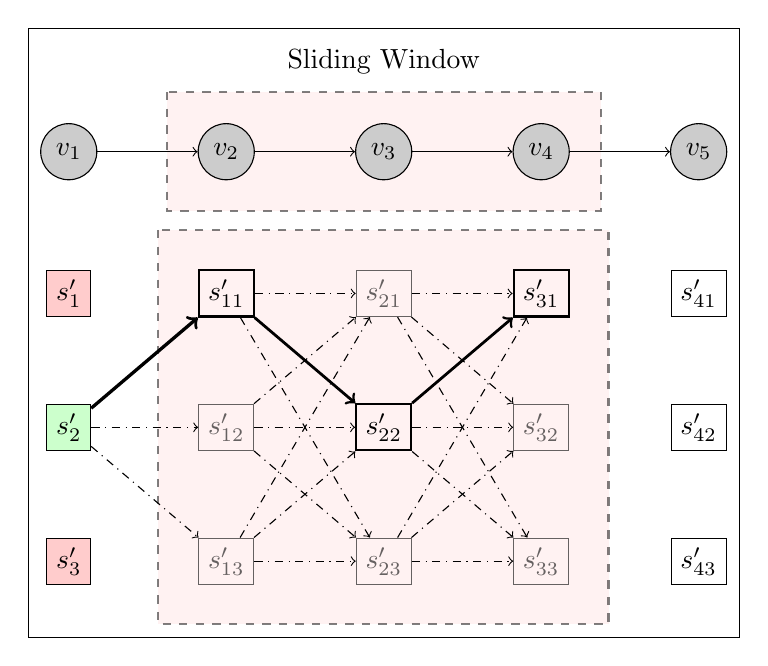
\begin{tikzpicture}[framed]

          \node[draw, circle, fill=gray!40,minimum width=0.7cm] (v1) at (1,5.2) {$\vi{1}$};
          \node[draw, circle, fill=gray!40,minimum width=0.7cm] (v2) at (3,5.2) {$\vi{2}$};
          \node[draw, circle, fill=gray!40,minimum width=0.7cm] (v3) at (5,5.2) {$\vi{3}$};
          \node[draw, circle, fill=gray!40,minimum width=0.7cm] (v4) at (7,5.2) {$\vi{4}$};
          \node[draw, circle, fill=gray!40,minimum width=0.7cm] (v5) at (9,5.2) {$\vi{5}$};
          \node[above, shift=({0,0.5}),  ] at (v3.north)  {Sliding Window};

          \node[draw, rectangle,fill=red!20] (s1) at (1,3.4) {$\sii{1}$};
          \node[draw, rectangle, fill=green!20] (s2) at (1,1.7) {$\sii{2}$};
          \node[draw, rectangle, fill=red!20] (s3) at (1,0) {$\sii{3}$};

          \node[draw, rectangle,thick] (s11) at (3,3.4) {$\sii{11}$};
          \node[draw, rectangle,opacity=.6] (s12) at (3,1.7) {$\sii{12}$};
          \node[draw, rectangle,opacity=.6] (s13) at (3,0) {$\sii{13}$};

          \node[draw, rectangle,opacity=.6] (s21) at (5,3.4) {$\sii{21}$};
          \node[draw, rectangle,thick] (s22) at (5,1.7) {$\sii{22}$};
          \node[draw, rectangle,opacity=.6] (s23) at (5,0) {$\sii{23}$};

          \node[draw, rectangle, thick] (s31) at (7,3.4) {$\sii{31}$};
          \node[draw, rectangle,opacity=.6] (s32) at (7,1.7) {$\sii{32}$};
          \node[draw, rectangle,opacity=.6] (s33) at (7,0) {$\sii{33}$};

          \node[draw, rectangle] (s41) at (9,3.4) {$\sii{41}$};
          \node[draw, rectangle] (s42) at (9,1.7) {$\sii{42}$};
          \node[draw, rectangle] (s43) at (9,0) {$\sii{43}$};

          \draw[->,line width= 1.2pt] (s2) -- (s11);
          \draw[->,dashdotted] (s2) -- (s12);
          \draw[->,dashdotted] (s2) -- (s13);

          \draw[->,line width= 1pt] (s11) -- (s22);

          \draw[->,dashdotted] (s11) -- (s21);
          \draw[->,dashdotted] (s11) -- (s23);

          \draw[->,dashdotted] (s12) -- (s21);
          \draw[->,dashdotted] (s12) -- (s22);
          \draw[->,dashdotted] (s12) -- (s23);

          \draw[->,dashdotted] (s13) -- (s21);
          \draw[->,dashdotted] (s13) -- (s22);
          \draw[->,dashdotted] (s13) -- (s23);

          \draw[->,dashdotted] (s21) -- (s31);
          \draw[->,dashdotted] (s21) -- (s32);
          \draw[->,dashdotted] (s21) -- (s33);

          \draw[->,line width=1pt] (s22) -- (s31);
          \draw[->,dashdotted] (s22) -- (s32);
          \draw[->,dashdotted] (s22) -- (s33);

          \draw[->,dashdotted] (s23) -- (s31);
          \draw[->,dashdotted] (s23) -- (s32);
          \draw[->,dashdotted] (s23) -- (s33);

          \draw[->] (v1) -- (v2);
          \draw[->] (v2) -- (v3);
          \draw[->] (v3) -- (v4);
          \draw[->] (v4) -- (v5);

          \begin{scope}[on background layer]
            \draw[thick, dashed, fill=red!10, opacity=0.5]
            ([shift={(-0.5,0.5)}]s11.north west) rectangle ([shift={(0.5,-0.5)}]s33.south east);

          \end{scope}
          \begin{scope}[on background layer]
            \draw[thick, dashed, fill=red!10, opacity=0.5]
            ([shift={(-0.5,0.5)}]v2.north west) rectangle ([shift={(0.5,-0.5)}]v4.south east);

          \end{scope}

        \end{tikzpicture}
      }
      \caption{Execution example of the sliding window heuristic using v=5, s=3, \windowsize=3 at i=1 step.}
      \label{fig:execution_example}
    \end{figure}

    The simulator defines dependencies between filtering transformations made by candidate services at consecutive vertices of the pipeline template.
    To this aim, it assigns a dependency rate to each service \si{i} modeling the amount of the filtering transformation done at \si{i} that overlaps the one at \si{i-1}.
    For example, let us consider the pairs of services (\si{11},\si{21}) and (\si{11},\si{22}) with the following configurations: \emph{i)} service \si{11} introduces a filtering transformation that removes the 20\% of the dataset, \emph{ii)} service \si{21} introduces a filtering transformation that removes 10\% of the dataset and has dependency rate equal to 1, meaning that the filtering transformation made by \si{21} completely overlaps the one made by \si{11}, \emph{iii)} service \si{22} introduces a filtering transformation that removes 5\% of the dataset and has dependency rate equal to 0.5, meaning that the filtering transformation made by \si{22} overlaps half of the one made by \si{11}. Jaccard Metric $M_{J_{21}}$$=$0.8 at service \si{21}; $M_{J_{22}}$$=$0.775 at \si{22}, showing how dependencies can affect the pipeline quality and, in turn, the instantiation process.


    Our simulator also supports the comparison of the performance and quality of our sliding-window heuristic with \emph{i)} a baseline modeling solutions in the state of the art and \emph{ii)} the exhaustive approach (i.e., the theoretical optimum). We modeled our baseline as a greedy approach that, for each node of the service pipeline, selects the best service that maximizes the data quality, while addressing data protection requirements in annotation $\myLambda$. The reason is that, to the best of our knowledge, existing (industry) solutions and standards do not support service-based data pipelines and are therefore unable to instantiate the service pipeline according to the pipeline structure and service dependencies. We therefore defined our baseline as the sliding window heuristic configured with window size $|$w$|$=1.
    We implemented the exhaustive approach calculating the theoretical optimum as the sliding window heuristic configured with window size $|$w$|$=$l$, to illustrate the potential efficiency of our heuristics within realistic computational limits.

    \begin{table}[!t]
      \caption{Experimental Parameters}
      \label{tab:parameters}
      \centering
      {\color{OurColor2}
        \begin{tabular}{l|l}
          \textbf{Parameter}                   & \textbf{Values}                               \\
          \hline
          Window Size \textbar{}w\textbar{}    & 1, 2, 3, 4, 5, 6, 7                           \\
          Pipeline Template Length $l$         & 3, 4, 5, 6, 7                                 \\
          Number of Candidate Services $|S^c|$ & 2, 3, 4, 5, 6, 7                              \\
          Filtering Configuration              & wide, average                                 \\
          Metric                               & quantitative ($M_J$), qualitative ($M_{JSD}$) \\
        \end{tabular}
      }
    \end{table}
    {\color{OurColor2}
    \cref{tab:parameters} outlines the parameters and corresponding values used in our experimental evaluation. Paremeter \emph{Window Size} (\textbar{}w\textbar{}), varying from 1 to 7, models different configurations of our heuristic. Parameter \emph{Pipeline Template Length $l$}, varying from 3 to 7, models the depth of the pipeline template as the number of vertices composed in a sequence. Parameter \emph{Number of Candidate Services $|S^c|$}, varying from 2 to 7, models the number of alternative services at each vertex of the pipeline template. Parameter \emph{Filtering Configuration} considers two representative filtering transformations: \textit{wide} removing a percentage of data in [0.2,1] and \textit{average} in [0.5,0.8]. Parameter \emph{Metric} considers two quality metrics: quantitative ($M_J$) and qualitative ($M_{JSD}$).}

    Our experiments have been run on a virtual machine equipped with an Intel(R) Xeon(R) CPU E5-2620 v4 @ 2.10GHz CPU and 32GB RAM. Each experiment was repeated 10 times and the results averaged to improve the reliability of findings.

    \begin{figure}[!ht]
      \centering
      \begin{subfigure}{0.45\textwidth}
        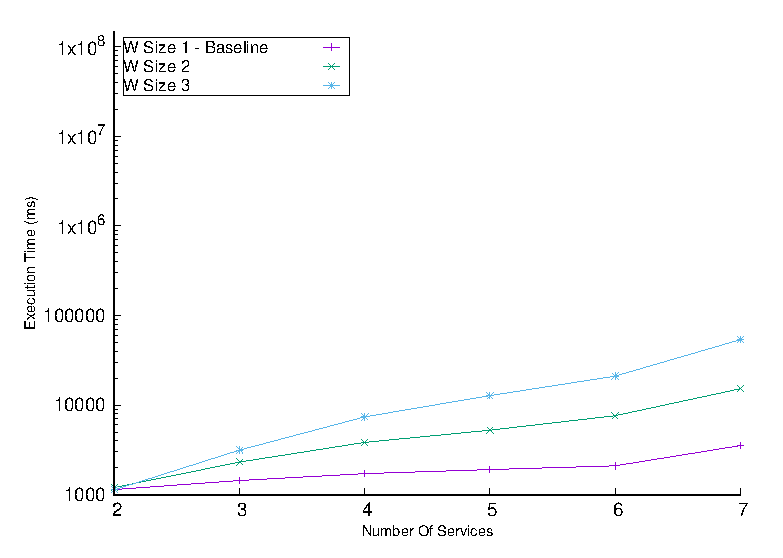
\includegraphics[width=\textwidth]{Images/graphs/window_time_performance_qualitative_n7_s7_50_80_n3}
        \caption{3 vertices}
        \label{fig:time_window_perce_wide_3n}
      \end{subfigure}
      \hfill
      \begin{subfigure}{0.45\textwidth}
        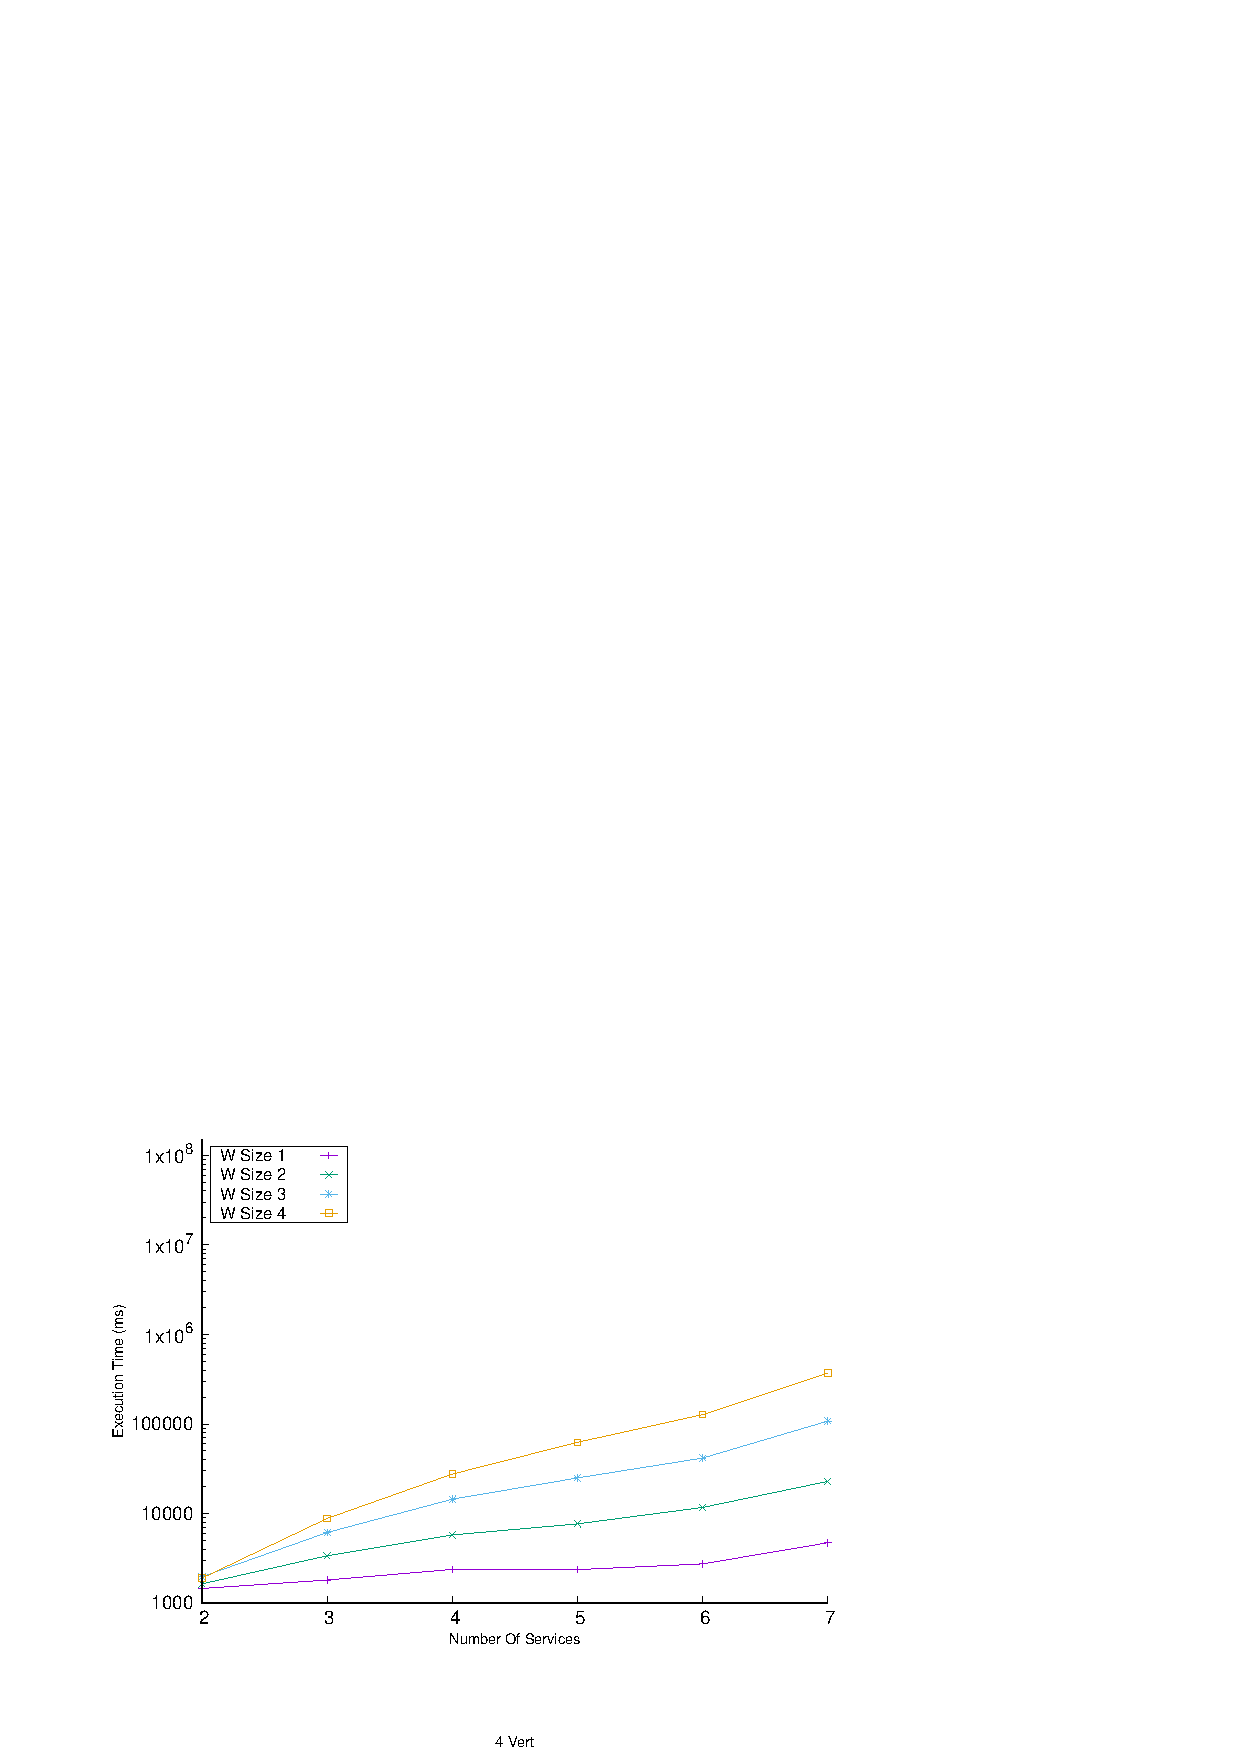
\includegraphics[width=\textwidth]{Images/graphs/window_time_performance_qualitative_n7_s7_50_80_n4}
        \caption{4 vertices}
        \label{fig:time_window_perce_wide_4n}
      \end{subfigure}
      \hfill
      \begin{subfigure}{0.45\textwidth}
        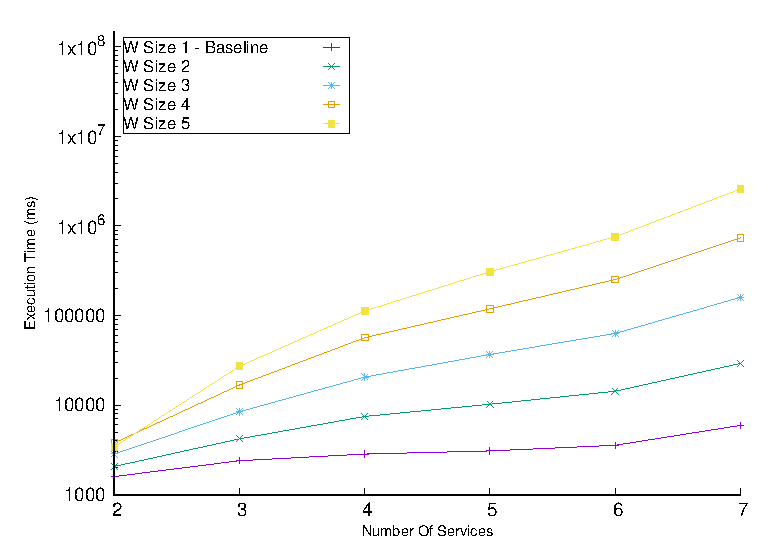
\includegraphics[width=\textwidth]{Images/graphs/window_time_performance_qualitative_n7_s7_50_80_n5}
        \caption{5 vertices}
        \label{fig:time_window_perce_wide_5n}
      \end{subfigure}
      \hfill
      \begin{subfigure}{0.45\textwidth}
        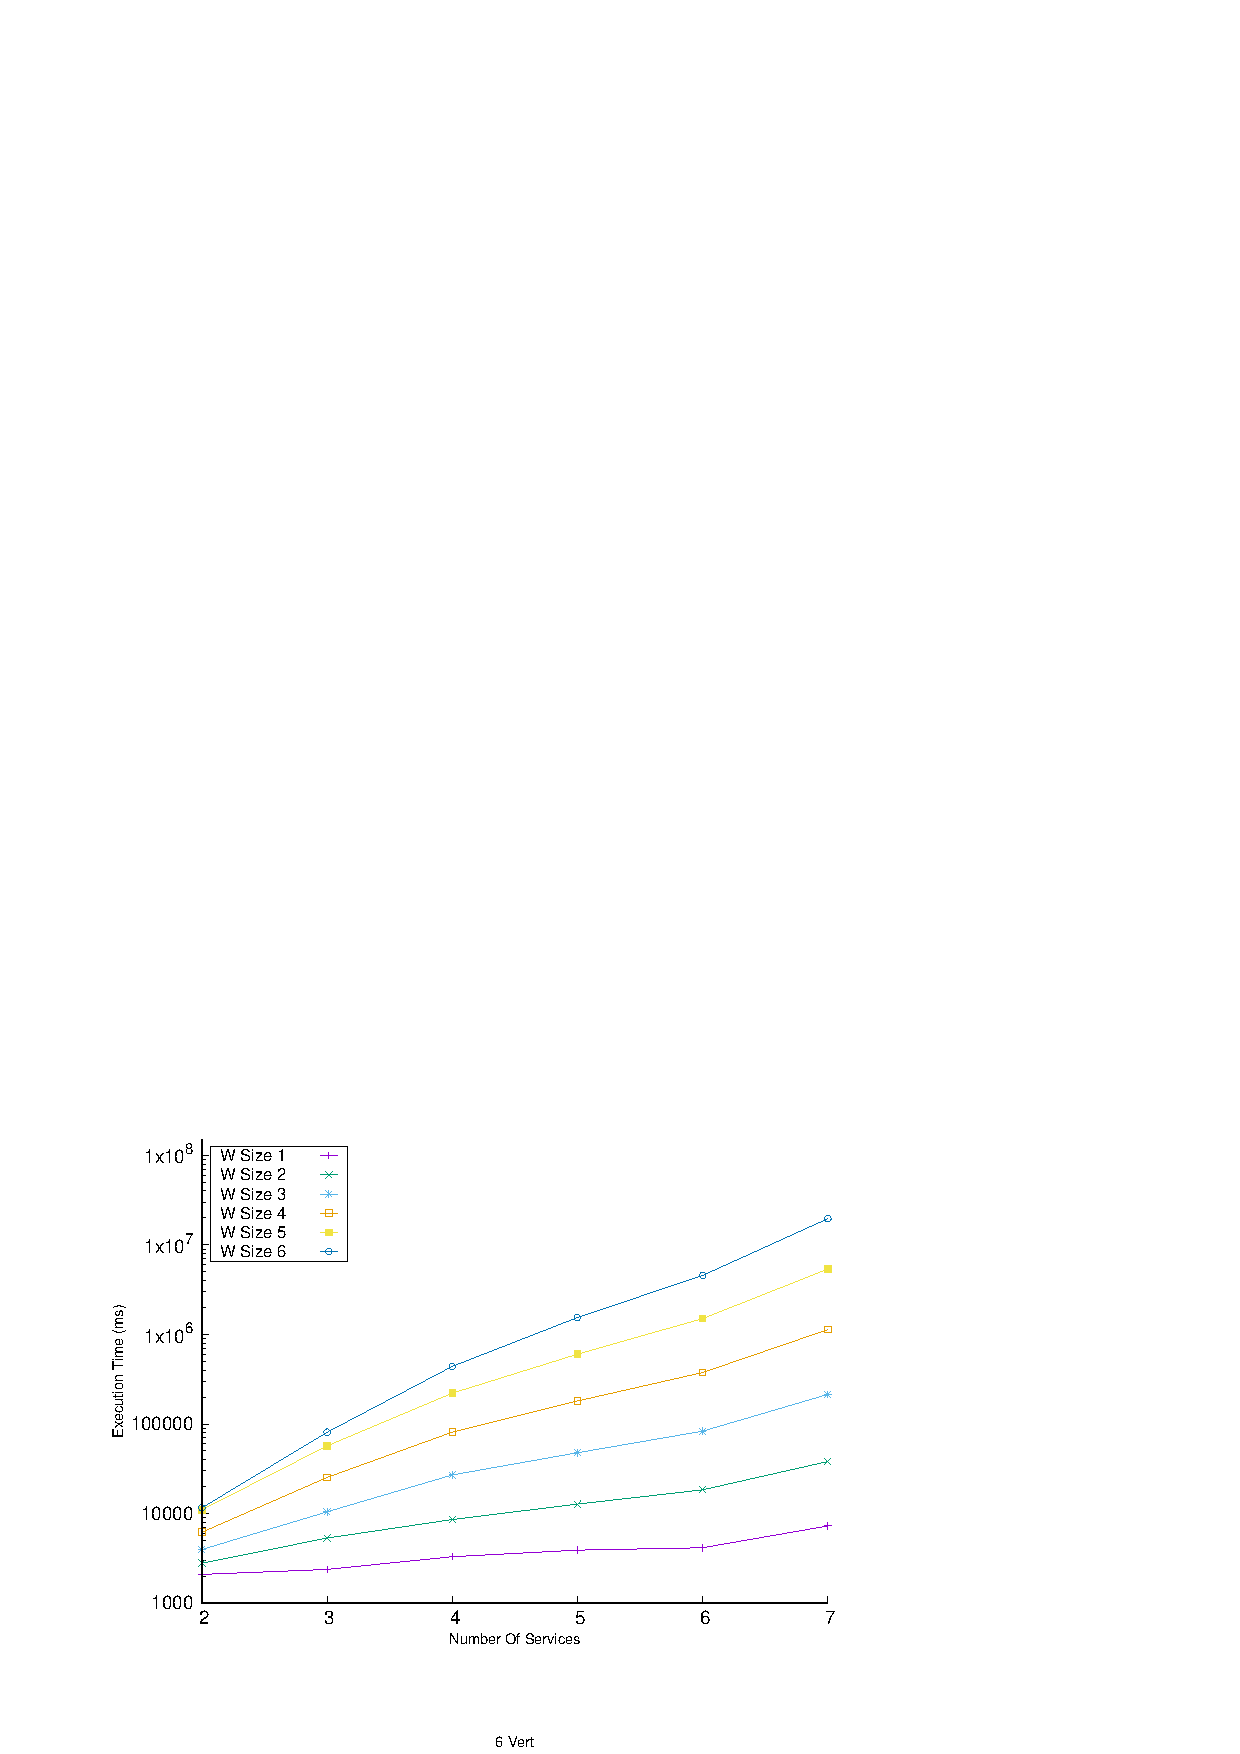
\includegraphics[width=\textwidth]{Images/graphs/window_time_performance_qualitative_n7_s7_50_80_n6}
        \caption{6 vertices}
        \label{fig:time_window_perce_wide_6n}
      \end{subfigure}
      \begin{subfigure}{0.45\textwidth}
        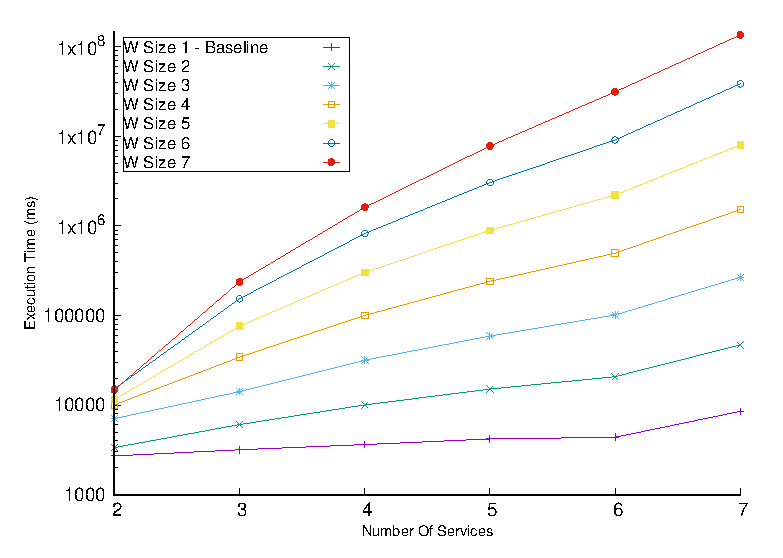
\includegraphics[width=\textwidth]{Images/graphs/window_time_performance_qualitative_n7_s7_50_80_n7}
        \caption{7 vertices}
        \label{fig:time_window_perce_wide_7n}
      \end{subfigure}
      \caption{{\color{OurColor2}Evaluation of Performance Using the \emph{Qualitative} Metric in
            Configuration \average}}
      \label{fig:time_window_perce_average}
    \end{figure}
    \subsection{Performance}\label{subsec:experiments_performance}
    We first measured the performance (execution time) of our exhaustive, baseline, and heuristic solutions by varying the pipeline template length $l$ in [3, 7] and the number of candidate services $|S^c|$ in [2, 7]. \cref{fig:time_window_perce_average} presents our results.
    The exhaustive approach can provide the optimal solution for all settings, but its execution time grows exponentially with the pipeline length and number of candidate services, making it impractical for large instances. For \windowsize\ from 1 to 3 (step 1), we observed a substantial reduction in execution time, with the heuristic always able to produce an instance in less than $\approx2.7\times10^5ms$ . The worst heuristic performance ($l$=7, $|S^c|$=7, \windowsize=6) is $\approx3.8\times10^7ms$, one order of magnitude lower than the best exhaustive performance ($l$=7, $|S^c|$=7, \windowsize=7) $\approx1.35\times10^8ms$. {\color{OurColor} As expected, the baseline (i.e., our heuristic with \windowsize$=$1) shows the best performance in all settings.}


    \subsection{Quality}\label{subsec:experiments_quality}
    We evaluated the quality of our heuristic algorithm with different \windowsize\ comparing its results with the baseline and, where possible, with the optimal solution retrieved by executing the exhaustive approach.
    The quality $Q$ of the heuristic has been normalized between 0 and 1 by dividing it by the quality $Q^*$ retrieved by the exhaustive approach.

    We run our experiments varying: \emph{i)} pipeline template length $l$ in [3, 7], \emph{ii)} the window size \windowsize\ in [1,$l$], and \emph{iii)} the number of candidate services $|S^c|$ in [2, 7]. Each vertex is associated with a (set of) policy that applies filtering configuration \wide (removing a percentage of data in $[0.2,1]$) or \average (removing a percentage of data in $[0.5,0.8]$).

    {\color{OurColor2}\cref{fig:quality_window_perce_average} presents} our quality results using metric $M_J$ in \cref{subsec:metrics} for configurations \wide and \average, respectively.
    In general, we observe that the quality of our heuristic approach increases as the window size increases, providing a quality comparable to the exhaustive approach when the window size \windowsize\ approaches the length $l$ of the pipeline template.

    When considering configuration \wide, the baseline (\windowsize=1) provides good results on average (0.71, 0.90), while showing substantial quality oscillations in specific runs: between 0.882 and 0.970 for pipeline template $l$=3, 0.810 and 0.942 for $l$=4, 0.580 and 0.853 for $l$=5, 0.682 and 0.943 for $l$=6, 0.596 and 0.821 for $l$=7. This same trend emerges when the window size is $<$$l$/2, while it starts approaching the optimum when the window size is $\geq$$l$/2. For instance, when \windowsize=$l$-1, the quality varies between 0.957 and 1.0 for $l$=3, 0.982 and 1.0 for $l$=4, 0.986 and 0.998 for $l$=5, 0.977 and 1.0 for $l$=6, 0.996 and 1.0 for $l$=7.
    \begin{figure}[ht]
      \centering
      \begin{subfigure}{0.49\textwidth}
        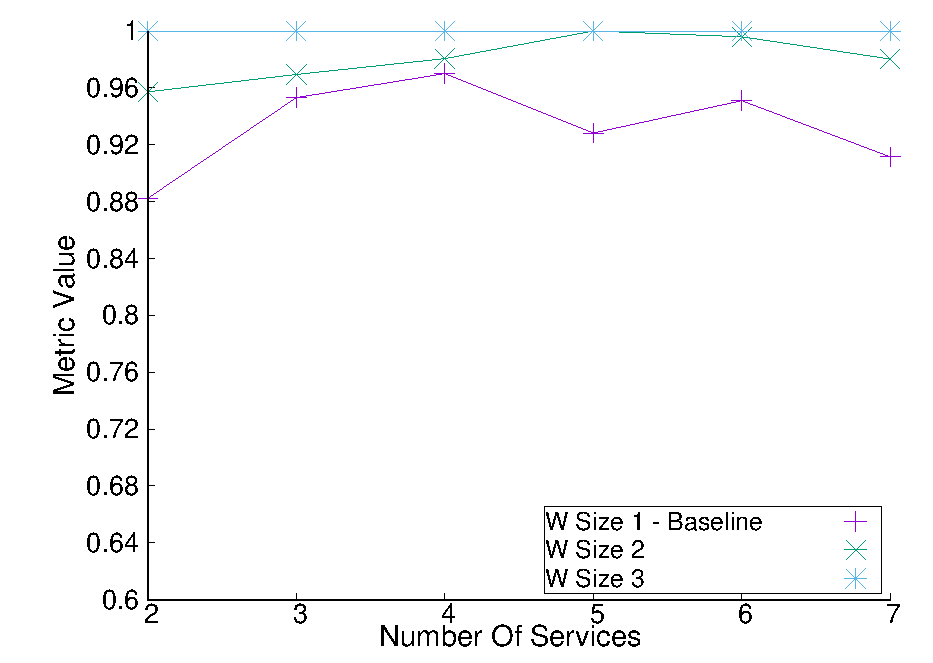
\includegraphics[width=\textwidth]{Images/graphs/window_quality_performance_diff_perce_n7_s7_20_100_n3}
        \caption{\wide 3 vertices}
        \label{fig:quality_window_wide_perce_n3}
      \end{subfigure}
      \hfill
      \begin{subfigure}{0.49\textwidth}
        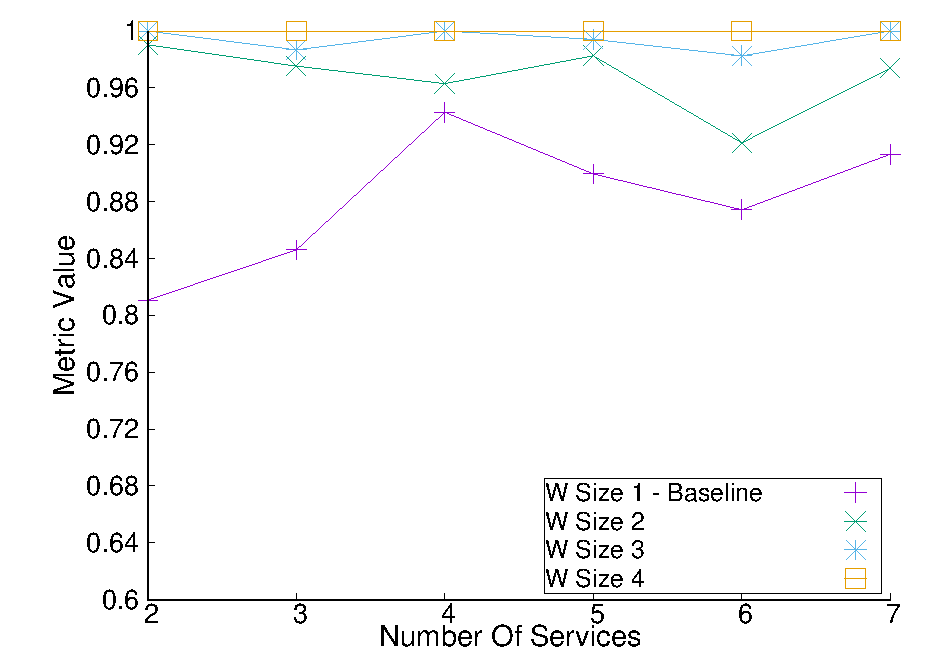
\includegraphics[width=\textwidth]{Images/graphs/window_quality_performance_diff_perce_n7_s7_20_100_n4}
        \caption{\wide 4 vertices}
        \label{fig:quality_window_wide_perce_n4}
      \end{subfigure}
      \hfill
      \begin{subfigure}{0.49\textwidth}
        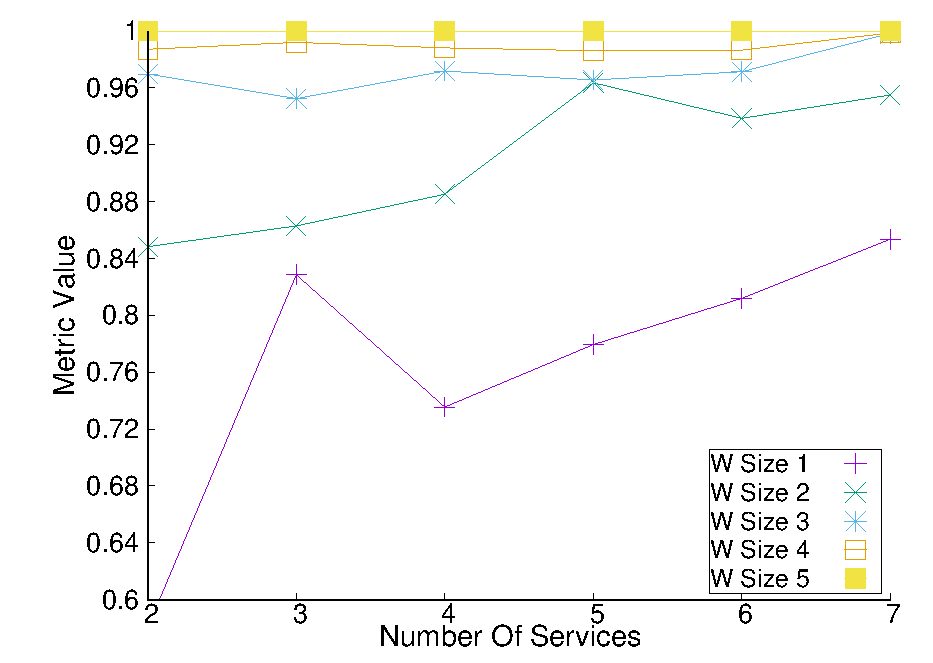
\includegraphics[width=\textwidth]{Images/graphs/window_quality_performance_diff_perce_n7_s7_20_100_n5}
        \caption{\wide 5 vertices}

        \label{fig:quality_window_wide_perce_n5}
      \end{subfigure}
      \hfill
      \begin{subfigure}{0.49\textwidth}
        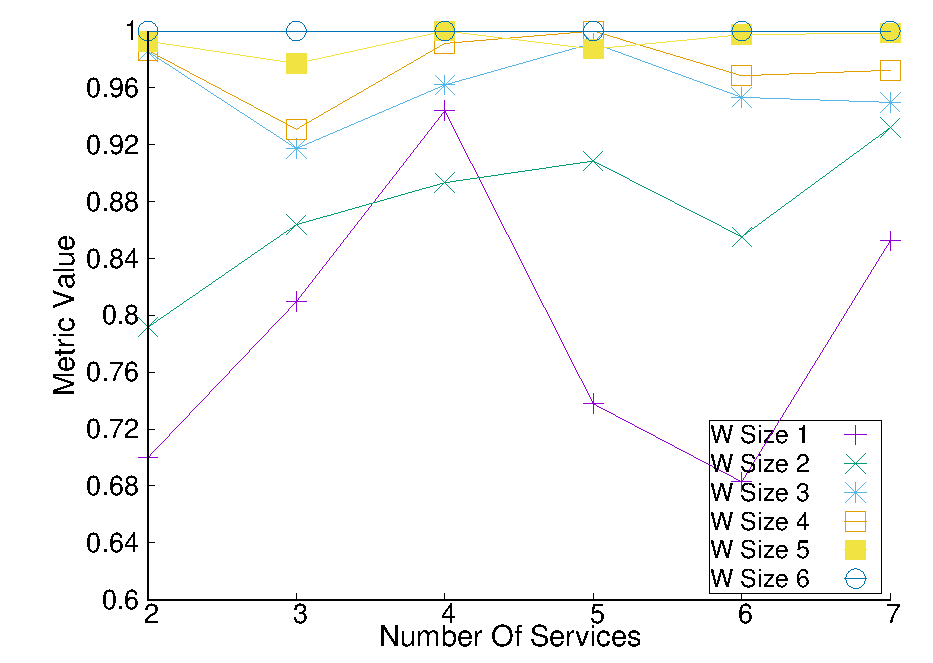
\includegraphics[width=\textwidth]{Images/graphs/window_quality_performance_diff_perce_n7_s7_20_100_n6}
        \caption{\wide 6 vertices}
        \label{fig:quality_window_wide_perce_n6}
      \end{subfigure}
      \hfill
      \begin{subfigure}{0.49\textwidth}
        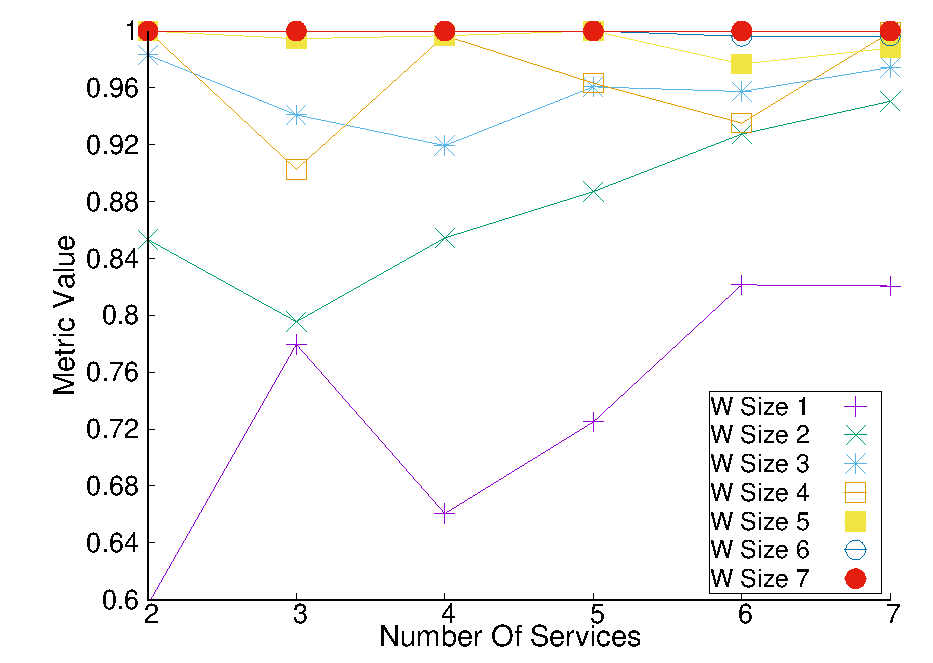
\includegraphics[width=\textwidth]{Images/graphs/window_quality_performance_diff_perce_n7_s7_20_100_n7}
        \caption{\wide 7 vertices}
        \label{fig:quality_window_wide_perce_n7}
      \end{subfigure}



      \caption{Evaluation of Quality Using the \emph{Quantitative} Metric in a \wide (\cref{fig:quality_window_wide_perce_n3,fig:quality_window_wide_perce_n4,fig:quality_window_wide_perce_n5,fig:quality_window_wide_perce_n6,fig:quality_window_wide_perce_n7}) Profile Configuration.}  \label{fig:quality_window_perce_wide}

    \end{figure}



    When considering configuration \average (\cref{fig:quality_window_perce_average}), the heuristic algorithm still provides good results, limiting the quality oscillations observed for configuration \wide\ and approaching the quality of the exhaustive also for lower window sizes. The baseline (\windowsize=1) provides good results on average (from 0.842 to 0.944), as well as in specific runs: between 0.927 and 0.978 for $l$=3, 0.903 and 0.962 for $l$=4, 0.840 and 0.915 for $l$=5, 0.815 and 0.934 for $l$=6, 0.721 and 0.935 for $l$=7.
    When \windowsize=$l$-1, the quality varies between 0.980 and 1.0 for $l$=3, 0.978 and 1.0 for $l$=4, 0.954 and 1 for $l$=5, 0.987 and 1.0 for $l$=6, 0.990 and 1.0 for $l$=7.

    \cref{fig:quality_window_perce_average,fig:quality_window_perce_wide} {\color{OurColor2}presents} our quality results using metric $M_{JSD}$ in \cref{subsec:metrics} for configurations \wide and \average, respectively.
    \begin{figure}[ht]
      \centering
      \begin{subfigure}{0.49\textwidth}
        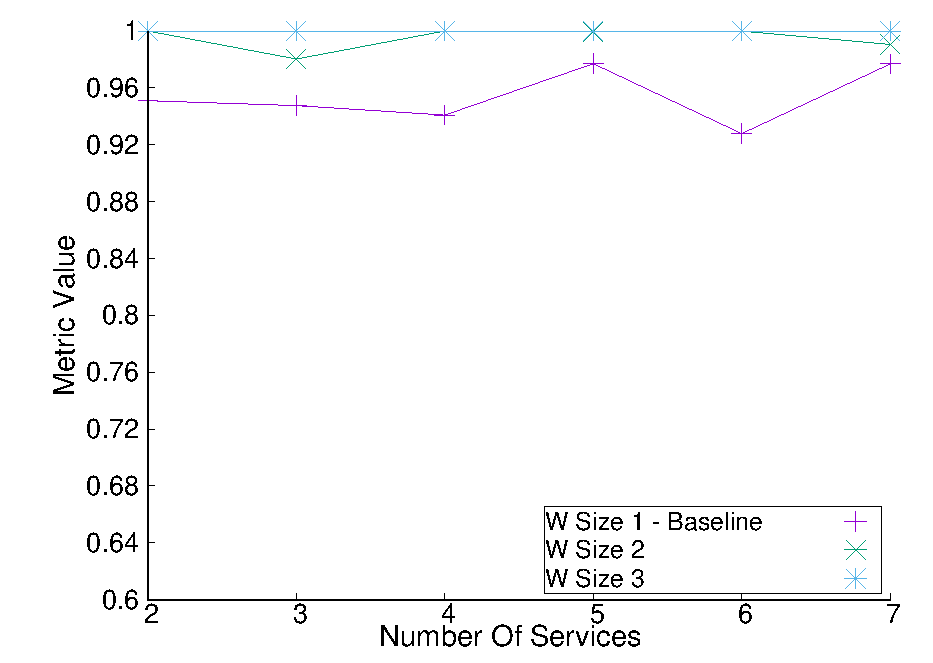
\includegraphics[width=\textwidth]{Images/graphs/window_quality_performance_diff_perce_n7_s7_50_89_n3}
        \caption{\average 3 vertices}

        \label{fig:quality_window_average_perce_n3}
      \end{subfigure}
      \hfill
      \begin{subfigure}{0.49\textwidth}
        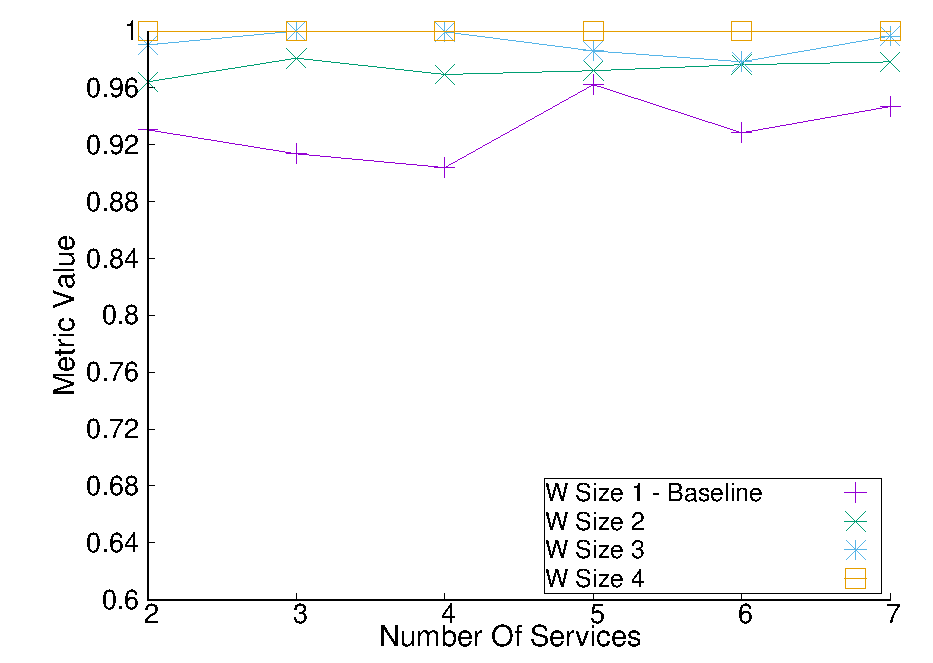
\includegraphics[width=\textwidth]{Images/graphs/window_quality_performance_diff_perce_n7_s7_50_89_n4}
        \caption{\average 4 vertices}

        \label{fig:quality_window_average_perce_n4}
      \end{subfigure}
      \hfill
      \begin{subfigure}{0.49\textwidth}
        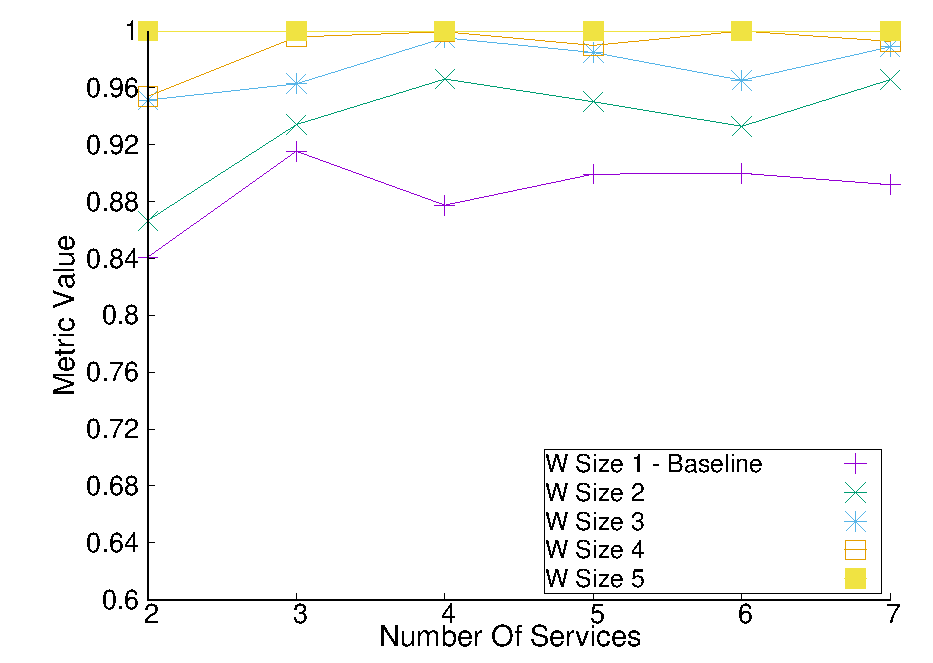
\includegraphics[width=\textwidth]{Images/graphs/window_quality_performance_diff_perce_n7_s7_50_89_n5}
        \caption{\average 5 vertices}
        \label{fig:quality_window_average_perce_n5}
      \end{subfigure}
      \hfill
      \begin{subfigure}{0.49\textwidth}
        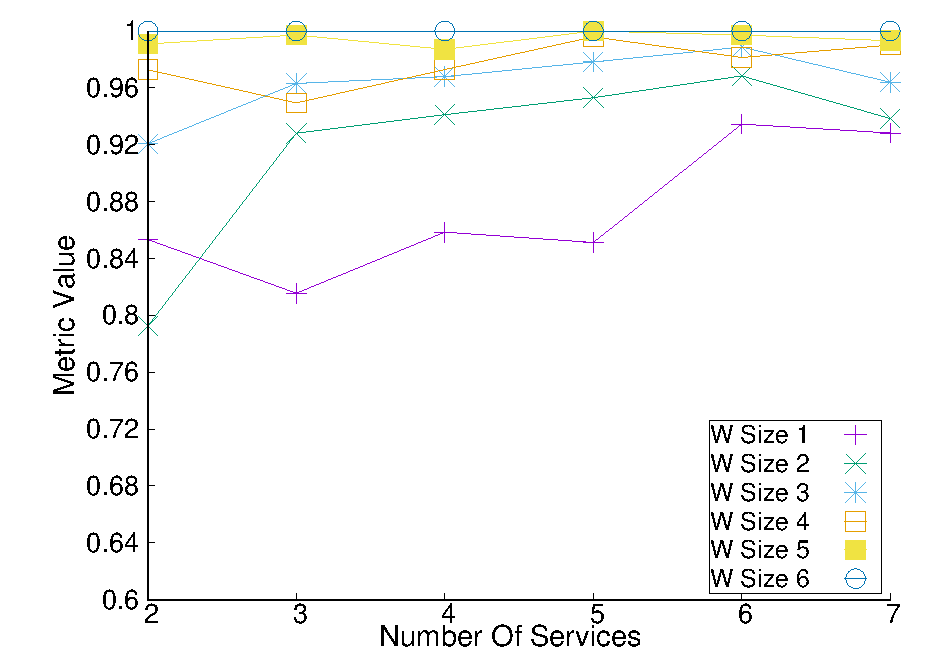
\includegraphics[width=\textwidth]{Images/graphs/window_quality_performance_diff_perce_n7_s7_50_89_n6}
        \caption{\average 6 vertices}
        \label{fig:quality_window_average_perce_n6}
      \end{subfigure}
      \hfill
      \begin{subfigure}{0.49\textwidth}
        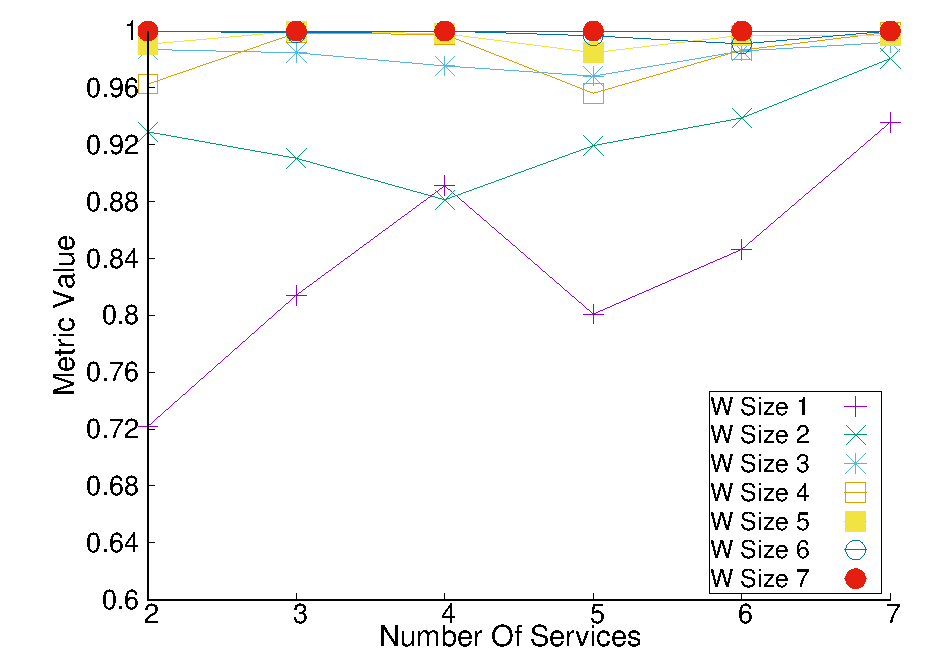
\includegraphics[width=\textwidth]{Images/graphs/window_quality_performance_diff_perce_n7_s7_50_89_n7}
        \caption{\average 7 vertices}
        \label{fig:quality_window_average_perce_n7}
      \end{subfigure}


      \caption{Evaluation of Quality Using the \emph{Quantitative} Metric in an \average (\cref{fig:quality_window_average_perce_n3,fig:quality_window_average_perce_n4,fig:quality_window_average_perce_n5,fig:quality_window_average_perce_n6,fig:quality_window_average_perce_n7}) Profile Configuration.}  \label{fig:quality_window_perce_average}

    \end{figure}

    %QUAAAAAAAAAAAAAAAAAAAA

    When considering configuration \wide, the baseline (\windowsize=1) provides good results on average (0.92, 0.97), limiting oscillations observed with metric $M_J$; for instance, the quality varies between 0.951 and 0.989 for $l$=3, 0.941 and 0.988 for $l$=4, 0.919 and 0.974 for $l$=5, 0.911 and 0.971 for $l$=6, 0.877 and 0.924 for $l$=7.
    The worst quality results are obtained with the baseline, while the oscillations are negligible when the window size is $>$2. For instance, when \windowsize=$l$-2, the quality varies between, 0.982 and 0.996 for $l$=4, 0.981 and 0.998 for $l$=5, 0.988 and 1.0 for $l$=6, 0.976 and 0.999 for $l$=7. When \windowsize=$l$-1, the quality varies between  0.987 and  0.998 for $l$=3, 0.993 and 1.0 for $l$=4, 0.985 and 0.999 for $l$=5, 0.997 and 1.0 for $l$=6, 0.995 and 1.0  for $l$=7.

    \begin{figure}[H]
      \centering
      \begin{subfigure}{0.49\textwidth}
        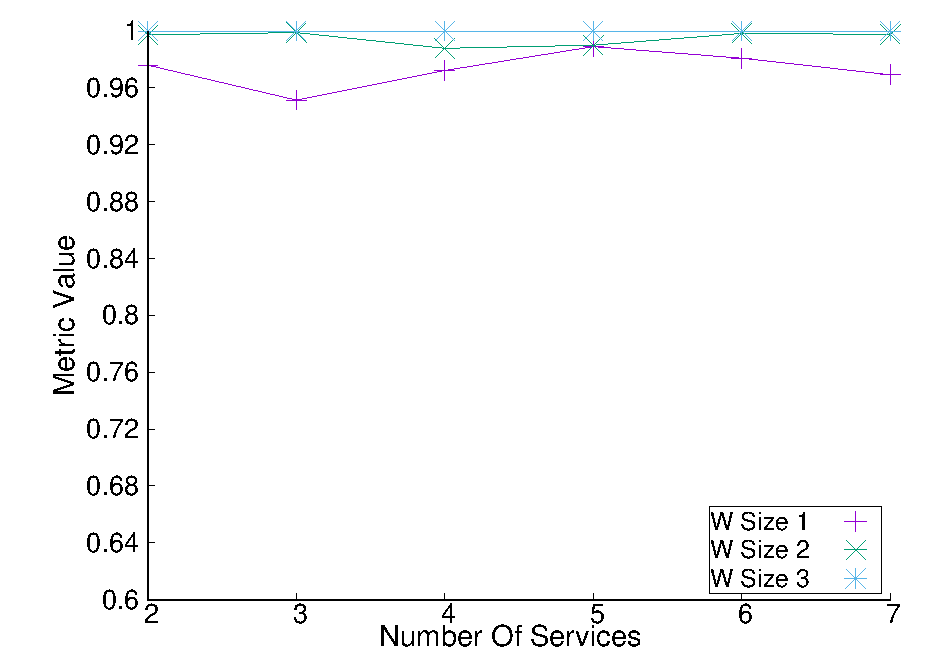
\includegraphics[width=\textwidth]{Images/graphs/window_quality_performance_diff_qual_n7_s7_20_100_n3}
        \caption{\wide 3 vertices}
        \label{fig:quality_window_wide_qualitative_n3}
      \end{subfigure}
      \hfill
      \begin{subfigure}{0.49\textwidth}
        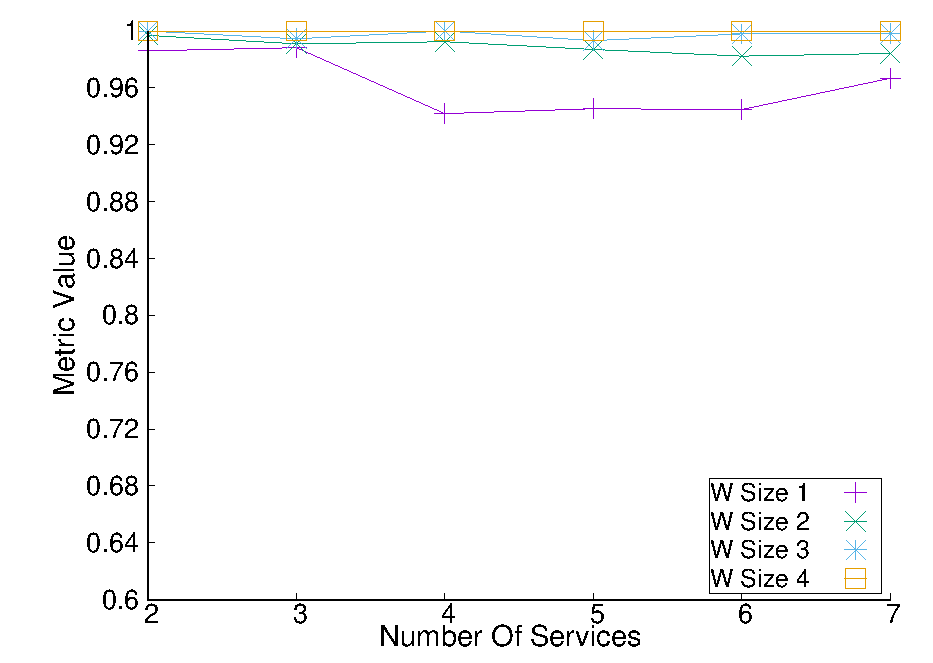
\includegraphics[width=\textwidth]{Images/graphs/window_quality_performance_diff_qual_n7_s7_20_100_n4}
        \caption{\wide 4 vertices}
        \label{fig:quality_window_wide_qualitative_n4}
      \end{subfigure}
      \hfill
      \begin{subfigure}{0.49\textwidth}
        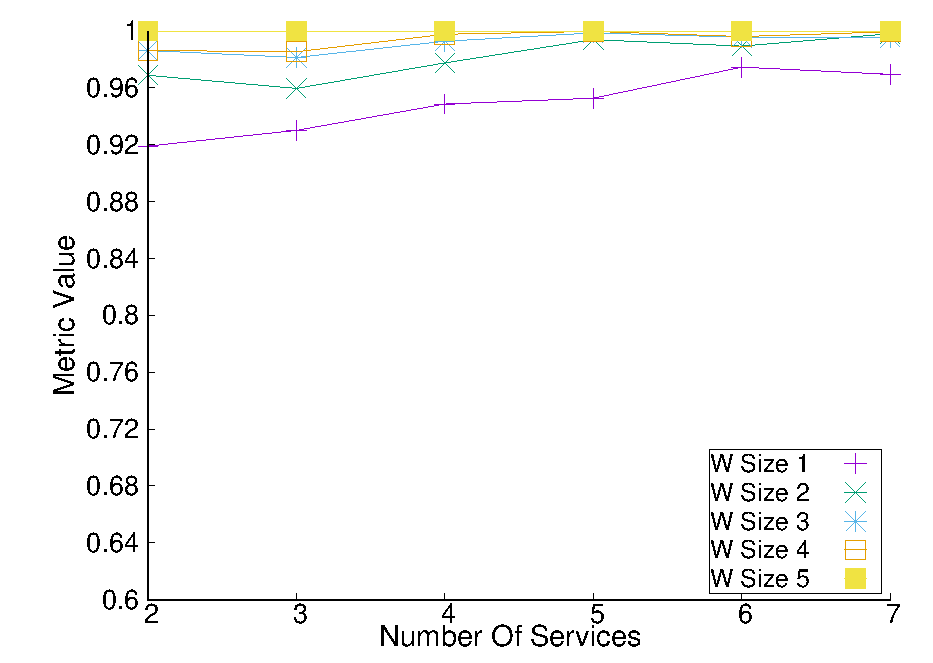
\includegraphics[width=\textwidth]{Images/graphs/window_quality_performance_diff_qual_n7_s7_20_100_n5}
        \caption{\wide 5 vertices}
        \label{fig:quality_window_wide_qualitative_n5}
      \end{subfigure}
      \hfill
      \begin{subfigure}{0.49\textwidth}
        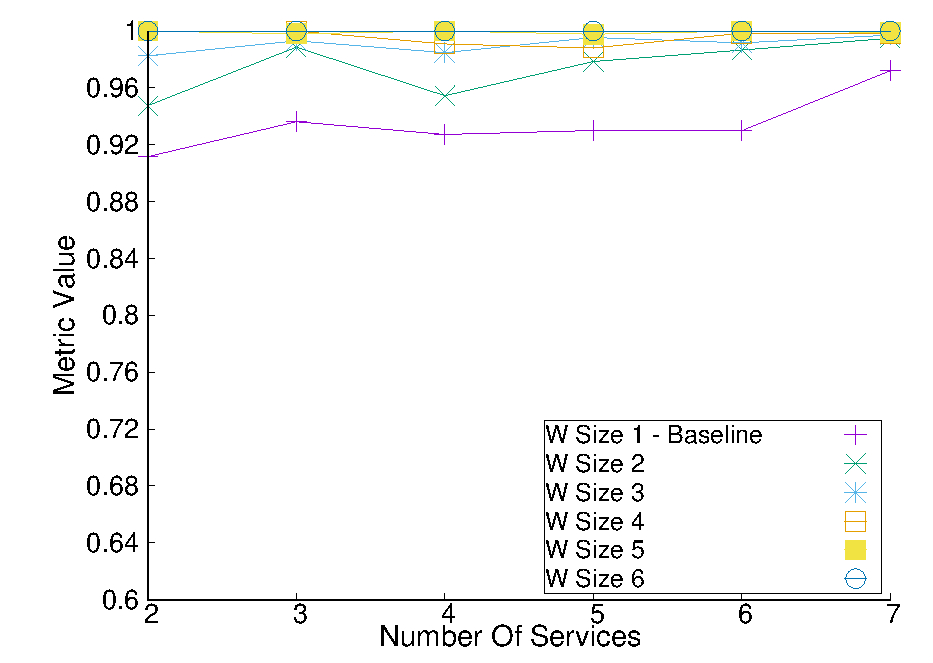
\includegraphics[width=\textwidth]{Images/graphs/window_quality_performance_diff_qual_n7_s7_20_100_n6}
        \caption{\wide 6 vertices}
        \label{fig:quality_window_wide_qualitative_n6}
      \end{subfigure}
      \hfill
      \begin{subfigure}{0.49\textwidth}
        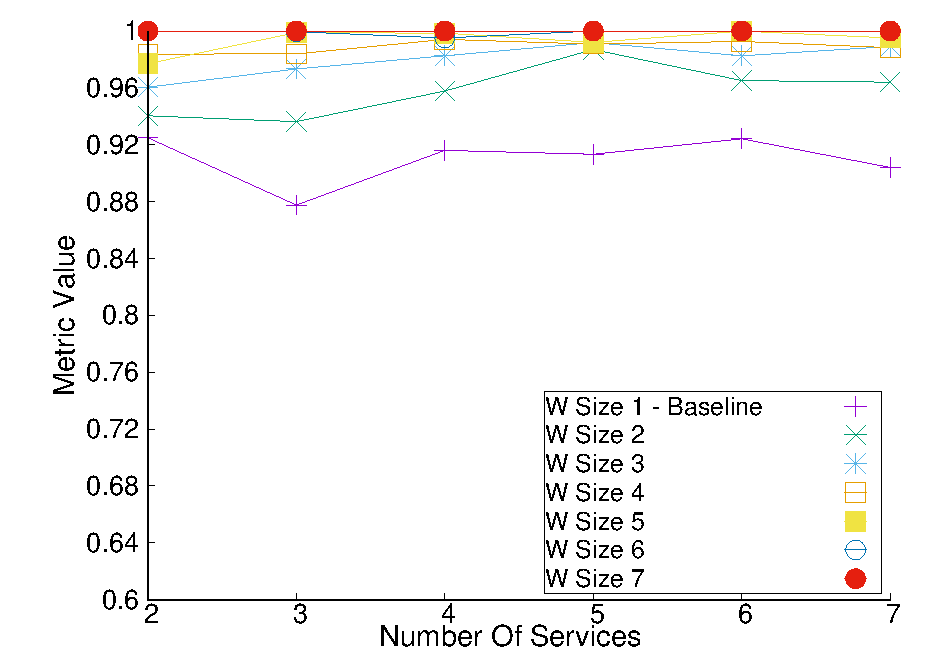
\includegraphics[width=\textwidth]{Images/graphs/window_quality_performance_diff_qual_n7_s7_20_100_n7}
        \caption{\wide 7 vertices}
        \label{fig:quality_window_wide_qualitative_n7}
      \end{subfigure}


      \caption{Evaluation of Quality Using the \emph{Qualitative} Metric in a \wide (\cref{fig:quality_window_wide_qualitative_n3,fig:quality_window_wide_qualitative_n4,fig:quality_window_wide_qualitative_n5,fig:quality_window_wide_qualitative_n6,fig:quality_window_wide_qualitative_n7}) Profile Configuration.}  \label{fig:quality_window_qualitative_wide}
    \end{figure}

    \begin{figure}[H]
      \centering
      \begin{subfigure}{0.49\textwidth}
        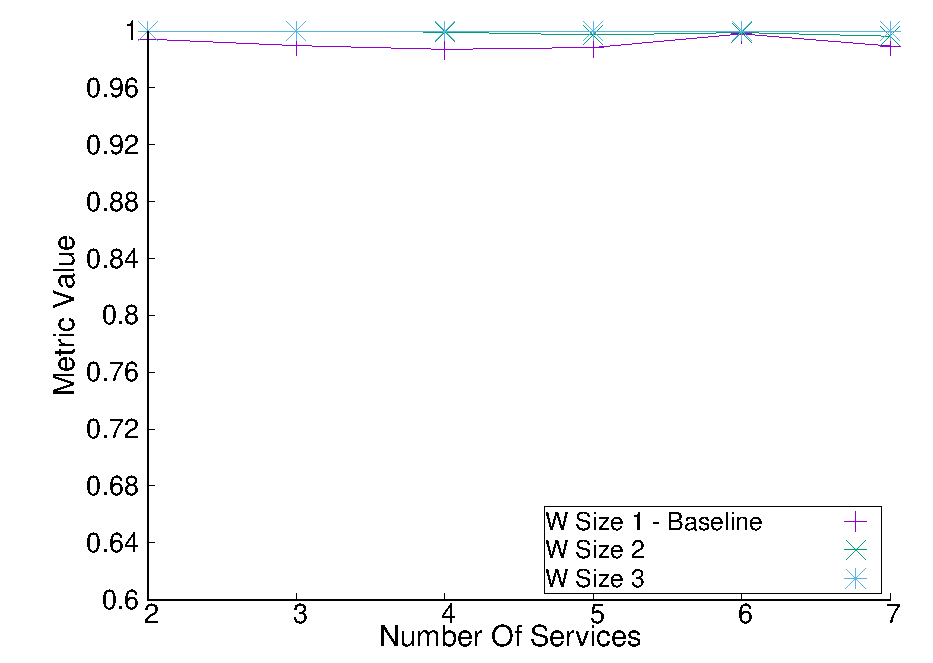
\includegraphics[width=\textwidth]{Images/graphs/window_quality_performance_diff_qual_n7_s7_50_80_n3}
        \caption{\average 3 vertices}
        \label{fig:quality_window_average_qualitative_n3}
      \end{subfigure}
      \hfill
      \begin{subfigure}{0.49\textwidth}
        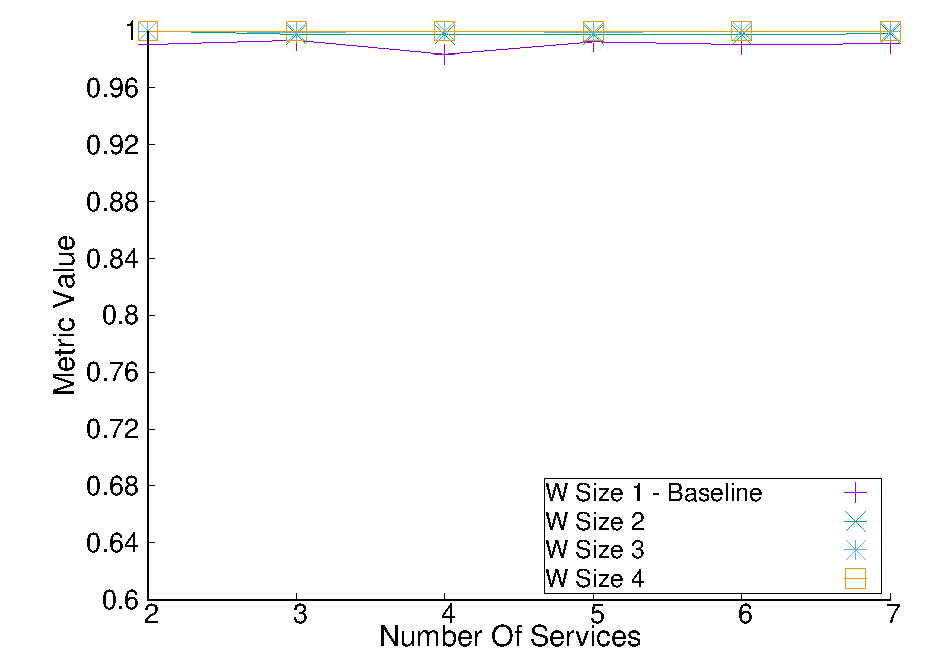
\includegraphics[width=\textwidth]{Images/graphs/window_quality_performance_diff_qual_n7_s7_50_80_n4}
        \caption{\average 4 vertices}
        \label{fig:quality_window_average_qualitative_n4}
      \end{subfigure}
      \hfill
      \begin{subfigure}{0.49\textwidth}
        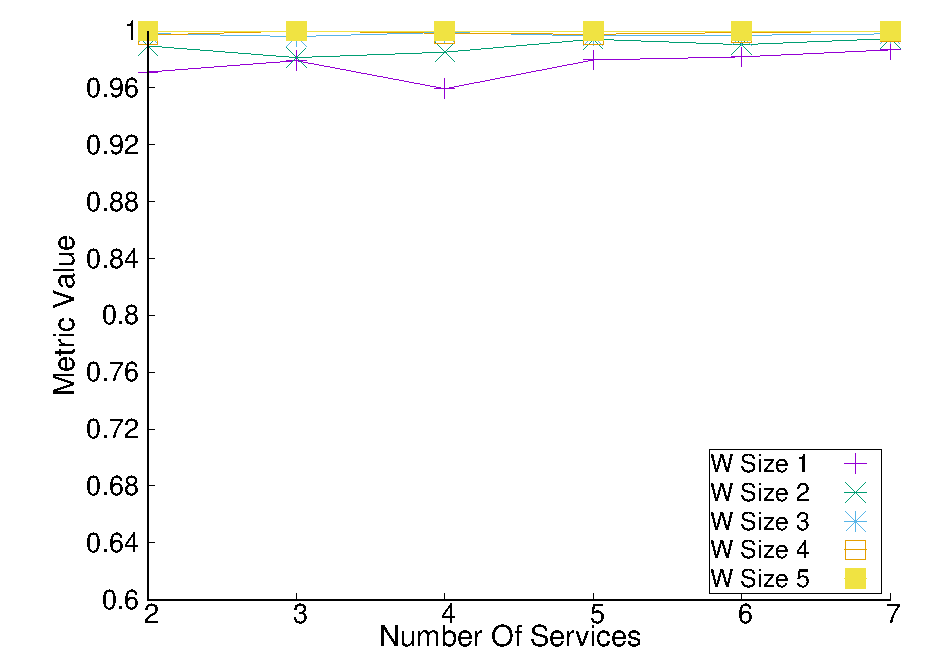
\includegraphics[width=\textwidth]{Images/graphs/window_quality_performance_diff_qual_n7_s7_50_80_n5}
        \caption{\average 5 vertices}
        \label{fig:quality_window_average_qualitative_n5}
      \end{subfigure}
      \hfill
      \begin{subfigure}{0.49\textwidth}
        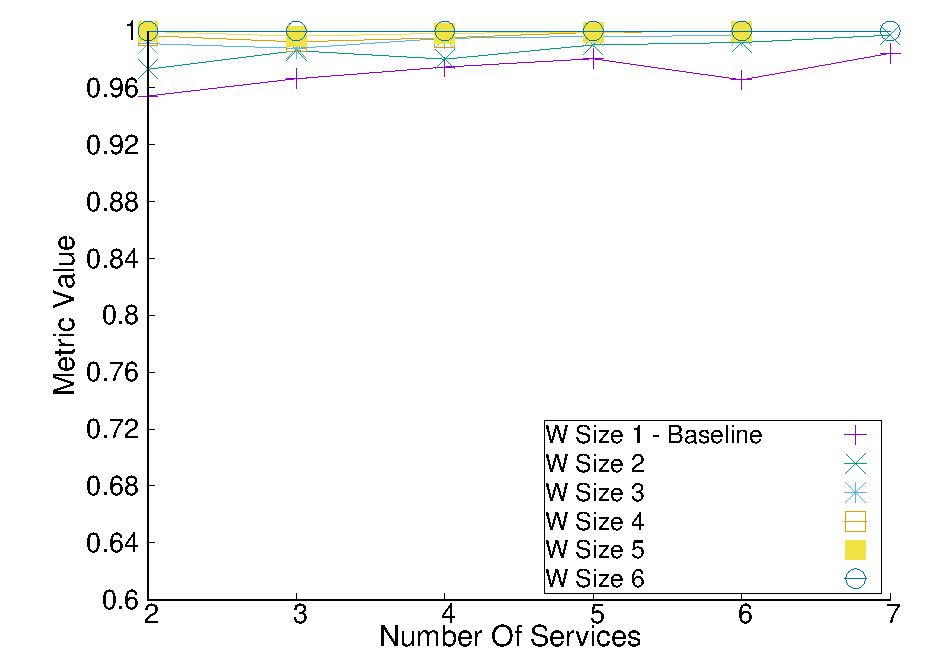
\includegraphics[width=\textwidth]{Images/graphs/window_quality_performance_diff_qual_n7_s7_50_80_n6}
        \caption{\average 6 vertices}
        \label{fig:quality_window_average_qualitative_n6}
      \end{subfigure}
      \hfill
      \begin{subfigure}{0.49\textwidth}
        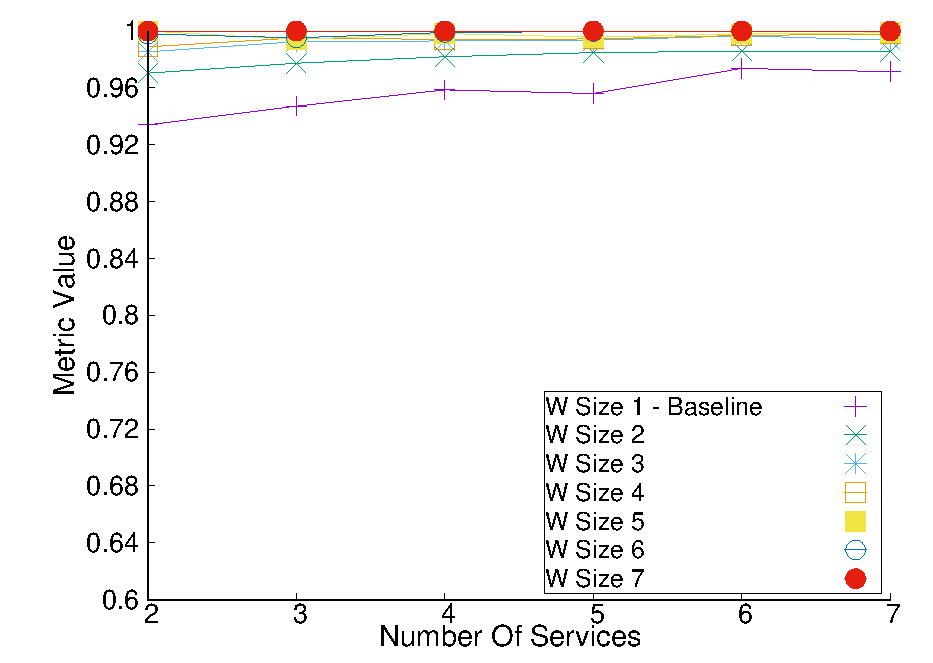
\includegraphics[width=\textwidth]{Images/graphs/window_quality_performance_diff_qual_n7_s7_50_80_n7}
        \caption{\average 7 vertices}
        \label{fig:quality_window_average_qualitative_n7}
      \end{subfigure}

      \caption{Evaluation of Quality Using the \emph{Qualitative} Metric in an \average (\cref{fig:quality_window_average_qualitative_n3,fig:quality_window_average_qualitative_n4,fig:quality_window_average_qualitative_n5,fig:quality_window_average_qualitative_n6,fig:quality_window_average_qualitative_n7}) Profile Configuration.}  \label{fig:quality_window_qualitative_average}

    \end{figure}

    When considering configuration \average, the baseline (\windowsize=1) provides results similar to configuration \wide. On average, quality varies from 0.920 to 0.969, limiting oscillations; for instance, the quality varies between 0.951 and 0.989 for $l$=3, 0.942 and 0.988 for $l$=4, 0.919 and 0.975 for $l$=5, 0.912 and 0.972 for $l$=6, 0.878 and 0.925 for $l$=7. The \average configuration provides even tighter quality oscillations than the \wide configuration. Notably, the poorest quality outcomes are observed with the baseline. Conversely, these oscillations become negligible when the window size exceeds 1 in configurations with three and four vertices, and when it exceeds 2 in configurations involving five, six, and seven vertices.  For instance, when \windowsize=3, the quality varies between  0.993 and 1 for $l$=4, 0.981 and 0.998 for $l$=5, 0.982 and 997 for $l$=6, 0.960 and 0.991 for $l$=7.


\subsection{Discussion}
The experimental results we obtained yield several valuable insights that merit further discussion. Three key observations emerged as follows.

\vspace{0.5em}

\noindent\textbf{Trade-off Between Execution Time and Quality.} As expected, the execution time improvement provided by our heuristic introduces a loss of quality with respect to the exhaustive approach. This loss causes an increase in the quality variance, especially when the window size (\windowsize) is small compared to the vertex count. A fine-grained tuning of heuristics is needed to balance computational efficiency and data quality.

\vspace{0.5em}

\noindent\textbf{Impact of Parameters on Quality.}
{\color{OurColor2}

  Our experiments demonstrate that parameters in Table~3 can significantly influence the quality of the pipeline, with the pipeline template length and the window size emerging as key factors for both quality and performance.

  Specifically, larger window sizes generally improve quality; however, there exists a balance point where the trade-off between computational cost and quality gain becomes suboptimal. Beyond this threshold, additional computational resources do not proportionately enhance data quality, as modeled by our metrics.
  We also note that lower window sizes exhibit higher instability, particularly under the \wide configuration, where data quality varies significantly across different setups. This variation diminishes when larger window sizes, approximately half the length of the pipeline (e.g., \windowsize$=$$l$/2), are used, leading to more stable and consistent results.

  We also note that the number of candidate services and service nodes increases the computation cost (performance) with a minor impact on quality (on average).

  In conclusion, our results demonstrate a significant reduction in computational overhead, while
  maintaining high data quality. Further analysis is needed to explore the impact of additional parameters, first of all in terms of diverse datasets modeling additional real-world domains, to understand their broader impact on quality. Investigating alternative quality metrics could also provide new insights and opportunities for improvement. Future experiments, as outlined in Section 9, will aim to address these aspects to provide a step further in the evaluation of the soundness and applicability of our framework on a larger scale.
}
\vspace{0.5em}

\noindent\textbf{Sliding Window Approach versus Global Awareness.} The intrinsic nature of our sliding window heuristic can sometimes lead to a local optimum, as the window size limits the candidate services for each pipeline stage to a restricted subset, which may prevent reaching the global optimum. This aspect is maximized when using the baseline representing the state of the art, where the sliding window heuristic is configured with a window size of \windowsize=1. Additionally, as dependencies between services increase, the likelihood of finding a sub-optimal solution rises. Our experiments show that \emph{i)} increasing the window size helps mitigate this issue and \emph{ii)} a broader decision-making scope becomes essential as service dependencies grow more complex.


\section{Related Work}\label{sec:related}


In this related work section, we address two fundamental challenges in the field of data protection for service-based pipelines. 
In Section  \ref{sec:dataquality}, we address the issue of the lack of consensus on the definition of data quality and, consequently, on data quality metrics when applying data protection transformations. In Section \ref{sec:datagov}, we examine existing data governance solutions that tackle the problem of data protection when sharing data among different services.

%%%%%%%%%%%%%%%%%%%%
\subsection{Data quality and data protection}\label{sec:dataquality}
%%%%%%%%%%%%%%%%%%%%

%Data quality is a widely studied research topic across various communities and perspectives, such as the database community or when evaluating privacy preserving data mining techniques. In the context of big data, data quality primarily refers to the extent to which big data meets the requirements and expectations of its intended use, encompassing various dimensions and characteristics to ensure the data is reliable, accurate, and valuable for analysis and decision-making. Specifically, accuracy denotes the correctness of the data, ensuring it accurately represents the real-world entities and events it models.
Data quality is a widely studied research topic studied across various communities and perspectives. In the context of (big) data pipelines, data quality primarily refers to the extent to which (big) data meets the requirements and expectations of its intended use, encompassing various dimensions and characteristics to ensure the data are reliable, accurate, and valuable for analysis and decision-making. Specifically, accuracy denotes the correctness of the data, ensuring it accurately represents the real-world entities and events it models.

With the increasing need to protect sensitive data, the notion of data quality has expanded to include a broader concept of accuracy, particularly in terms of the proximity of a sanitized value to the original value.
This shift has emphasized the need of metrics to assess the quality of data resulting from anonymization processes. 
Differential privacy \cite{dwork2008differential}, k-anonymity \cite{k-anon}, and l-diversity \cite{l-diversity} are three distinct techniques used to provide data anonymization, with different protection levels and results on data quality. For example, differential privacy is highly effective in maintaining confidentiality, but the noise added can reduce data precision, impacting analytical accuracy, whereas k-anonymity and l-diversity generally maintain higher data quality than differential privacy, but they might still be unable to protect against sophisticated attacks.

Various data quality metrics have been proposed in existing literature, including generalized information loss (\textit{GenILoss}), discernability metric, minimal distortions, and average equivalence class size ($C_{AVG}$), which may either have broad applicability or be tailored to specific data scenarios \cite{Majeed2021AnonymizationTF,bookMetrics,reviewMetrics}. However, there is currently no metric that is widely accepted by the research community. The main challenge with data quality is its relative nature: its evaluation typically depends on the context in which the data is used and often involves both objective and subjective parameters \cite{dataAccuracy,dataQuality}.
%
A common consideration across all contexts is that accuracy is closely related to the information loss resulting from the anonymization strategy: the lower the information loss, the higher the data quality. In our scenario, we have opted for two generic metrics rooted in data loss assessment (i.e., data completeness) - one quantitative and one qualitative. Nonetheless, our framework and heuristic are designed to be modular and flexible, accommodating the chosen metric.

{\color{OurColor} While existing techniques have provided sound and effective solutions that guarantees data quality and data protection, they often unsuit to scenarios aiming to maximize data quality while ensuring data protection, have limited expressiveness (e.g., the definition of $k$ when $k$-anonymity is used to protect data), are not applicable to pipelines orchestrating services owned by different providers. Our solution fills in the above gaps, by providing a framework for service-based data pipelines that support the selection of data processing services that maximize data quality, while upholding privacy and security requirements. Service selection is driven by high-expressive policies, where data transformations built on data protection techniques (e.g., $k$-anonymity) are applied to data before they are used in the pipeline.} 

%%%%%%%%%%%%%%%%%%
\subsection{Data quality and data protection in service-based pipelines}\label{sec:datagov}
%%%%%%%%%%%%%%%%%%

As organizations increasingly realize the practical benefits and significant value of big data, they also acknowledge the limitations of current big data ecosystems, especially in terms of data governance. In this context, the need for privacy-aware systems enforcing sensitive data protection without compromising data quality throughout the entire data lifecycle arises. Recently, both industry and academia have begun to investigate the issue, recognizing the need of new security requirements \cite{Colombo:JournCybersec:2019} and the importance of addressing the conflict between the need to share and the need to protect information \cite{balancingact,VANDENBROEK2018330,balancingInMedicine,needtobalance,dataProtection}, from a data governance perspective \cite{al2018exploring,aissa2020decide}, and, more in general, to ensure compliance of (big) data pipelines with generic non-functional requirements \cite{ABBJ.ICWS2022,ABHKKS.BD2023}.

The pipeline template proposed in this work addresses these challenges by enabling to express the security policies at the right level of granularity, considering individual services in the pipeline. It can also be easily mapped onto specific platforms, such as Apache-based systems, as we have demonstrated in \cite{medes2021}.
Table \ref{tab:comparative} provides a comparative analysis with relevant existing approaches, highlighting how few industrial solutions compare to our framework according to the following critical features:
\begin{itemize}
    \item \textbf{F1 -- Service-Based Pipeline Support in the Cloud-Edge Continuum:} The ability to effectively operate within distributed environments spanning cloud and edge infrastructure.
    \item \textbf{F2 -- Quality-Aware Service Selection Ensuring Data Protection:} The capacity to optimize service selection processes, maintaining data quality across the pipeline and ensuring robust data protection measures.
    \item \textbf{F3 -- Framework-Agnostic Data Protection:} The degree to which each solution is bound to specific data protection techniques. 
    \item \textbf{F4 -- Policy Expressiveness:} The degree to which each solution supports fine-grained specification of policies or privacy measures.
\end{itemize}

\begin{table}[t!]
    \centering
    \renewcommand{\arraystretch}{1.5}
    \resizebox{\textwidth}{!}{%
    \begin{tabular}{lp{3cm}p{3.5cm}p{3cm}p{3cm}p{2.5cm}}
        \toprule
        \textbf{Solution} & \textbf{F1} & \textbf{F2} & \textbf{F3} & \textbf{F4} \\
        \midrule
        \textbf{Microsoft Presidio \cite{microsoft_presidio}} & \cmark, can integrate within cloud-edge pipelines & \tmark, focuses on data redaction & \cmark, compatible with diverse techniques & \tmark, pre-built PII detectors with configurable policies \\

        \textbf{Apache Ranger \cite{apache_ranger}} & \tmark, limited to mostly cloud settings & \xmark, provides access control rather than service optimization & \cmark, integrates with various techniques & \cmark; high expressiveness with fine-grained policy control \\

        \textbf{Our paper} & \cmark, suitable for cloud-edge environments & \cmark, enables selection of services that optimize data quality while ensuring data protection & \cmark, data-protection techniques agnostic & \cmark; high expressiveness with fine-grained policy control \\
        \bottomrule
    \end{tabular}
    }
    \caption{Comparative analysis with relevant existing approaches}
    \label{tab:comparative}
\end{table}

Additional solutions address individual aspects of these requirements. For example, several proposals address data protection by implementing robust access control on big data platforms. Some approaches are platform-specific, tailored to single systems like MongoDB or Hadoop, and leverage the native access control features of these platforms \cite{rathore2017hadoop,anisetti2018privacy,FederationAC:Journ:2020,Sandhu:ABAC:2018,GuptaSandu:2017}. Other approaches focus on specific databases, such as NoSQL or graph databases, or specific types of analytical pipelines \cite{AConGraphDB:2021, AConMongoDB:2022, ABACforHBase:2019}. However, these solutions often rely on query rewriting mechanisms, resulting in high complexity and low efficiency. Some solutions are designed for specific scenarios, such as federated cloud environments, edge microservices, or IoT, and lack the flexibility to adapt to multiple contexts \cite{MultipartyAC:2019, IoTSecurity}.
%
The most similar to our approach are platform-independent solutions that adopt Attribute-Based Access Control (ABAC) \cite{XACML3.0} as a common underlying model, given its ability to support highly flexible and dynamic forms of data protection for business-critical data. They have the advantage of being more general than platform-specific solutions, while they do not provide a complete framework like the one in this paper. 

To conclude, the selection and composition of services, originally discussed in the Web service scenario, face additional challenges in the era of big data due to the volume and velocity of data, as well as to the heterogeneity of services, domains, and hosting infrastructures. Despite its critical nature, security is often one of the least considered metrics in service selection \cite{SELLAMI2020102732}. Even when security is taken into account, it is not always coupled with data quality.
Related work in this area includes approaches (e.g., \cite{secureWScomposition}) where Web services are composed according to the security requirements of both service requestors and providers. However, the range of expressible requirements is limited, such as the type of encryption algorithm or authentication method (e.g., SSO), and data sanitization is not considered. Thus, the selection algorithm is just a matching rather than a ranking with respect to a security metrics.
Another relevant study \cite{9844845} implements a certification-based service selection process, ranking services according to their certified non-functional properties and corresponding user requirements. In this approach, certified services are assumed to be functionally equivalent, offering the same functionality while meeting users' functional requirements.
The most relevant solution is \cite{SELLAMI2020102732}, where the authors address the challenges of big service composition, with reference to QoS and security issues. Similarly to what we do with our pipeline template, they define a quality model for big services by extending the traditional QoS model of Web services to include ``big data"-related characteristics, and Quality of Data (QoD) attributes, such as completeness, accuracy, and timeliness. To address security issues, in their model, each service is assigned a L-Severity level \cite{Lseverity} that represents the potential severity of data leakages when consuming its data chunks.
Their approach aims to select the optimal composition plan that not only maximizes QoS and QoD attributes such as timeliness (TL), completeness (CP), and consistency (CS), but it also minimizes L-Severity (LS), data sources and communication costs.



\section{Conclusions}\label{sec:conclusions}
In the realm of distributed data service pipelines, managing pipelines while ensuring both data quality and data protection presents numerous challenges. This paper proposed a framework specifically designed to address this dual concern. Our data governance model employs policies and continuous monitoring to address data security and privacy challenges, while preserving data quality, in service pipeline generation. The key point of the framework is in its ability to annotate each element of the pipeline with specific data protection requirements and functional specifications, then driving service pipeline construction. This method enhances compliance with regulatory standards and improves data quality by preserving maximum information across pipeline execution. Experimental results confirmed the effectiveness of our sliding window heuristic in addressing the computationally complex NP-hard service selection problem at the basis of service pipeline construction. Making use of a realistic dataset, our experiments evaluated the framework's ability to sustain high data quality while ensuring robust data protection, which is essential for pipelines where both data utility and privacy must coexist. To fully understand the impact of dataset selection on the retrieved quality and to ensure heuristic robustness across various scenarios, further investigation is planned for our future work. Future work will then %validate the findings of this paper and
explore deeper insights into the applicability of our heuristics across different scenarios.

\section{Declarations}
\subsection{Ethics approval and consent to participate}
Not applicable
\subsection{Consent for publication}
Not applicable
\subsection{Availability of data and materials}
All data and materials are available at \url{https://github.com/SESARLab/Big-Data-Access-Control-Extension}
\subsection{Competing interests}
The authors declare that they have no competing interests.
\subsection{Funding}
Research supported, in parts, by \emph{i)} project ``BA-PHERD - Big Data Analytics Pipeline for the Identification of Heterogeneous Extracellular non-coding RNAs as Disease Biomarkers'', funded by the European Union - NextGenerationEU, under the National Recovery and Resilience Plan (NRRP) Mission 4 Component 2 Investment Line 1.1: “Fondo Bando PRIN 2022” (CUP G53D23002910006), \emph{ii)} project MUSA - Multilayered Urban Sustainability Action - project, funded by the European Union - NextGenerationEU, under the National Recovery and Resilience Plan (NRRP) Mission 4 Component 2 Investment Line 1.5: Strengthening of research structures and creation of R\&D ``innovation ecosystems'', set up of ``territorial leaders in R\&D'' (CUP  G43C22001370007, Code ECS00000037), \emph{iii)} project SERICS (PE00000014) under the
NRRP MUR program funded by the EU - NextGenerationEU, \emph{iv)} Università degli Studi di Milano under the program ``Piano di Sostegno alla Ricerca''. Views and opinions expressed are however those of the authors only and do not necessarily reflect those of the European Union or the Italian MUR. Neither the European Union nor the Italian MUR can be held responsible for them.
\subsection{Authors' contributions}
Marco Anisetti (M.A.) and Claudio A. Ardagna (C.A.A.) jointly conceived the original idea and guided the research direction. C.A.A., Chiara Braghin (C.B.), and Antongiacomo Polimeno (A.P.) developed the theoretical framework. A.P. was also responsible for conducting the experiments and drafting the whole manuscript, under the supervision of M.A., C.A.A., C.B.. All authors discussed the results, contributed to revisions of the manuscript, and approved the final version for publication.

\subsection{Acknowledgements}
Not applicable. No additional support was received from any individuals not listed as authors.

\clearpage
%\bibliographystyle{spbasic}      % basic style, author-year citations
%%%%%\bibliographystyle{spmpsci}      % mathematics and physical sciences
%\bibliographystyle{spphys}       % APS-like style for physics
\bibliography{bib_on_BigDataAccessControl}   % name your BibTeX data base

\end{document}

